\documentclass{beamer}
\usepackage[utf8]{inputenc}
\usepackage{amsmath, amssymb, bm}
\usepackage{physics}
\usepackage{graphicx}
\usepackage{hyperref}
\usepackage{xmpmulti}
\usepackage{tikz}
\usetheme{Madrid} % You can change the theme as you like
\usecolortheme{seagull}


\begin{document}

\title[Quantum Computing and ML]{\textbf{Quantum Technology and Artificial Intelligence}}
\author{Morten Hjorth-Jensen}
\institute{Department of Physics and Center for Computing in Science Education, University of Oslo, Norway}
\date{Sintef, COSY center seminar, May 12, 2025}


%-----------------------------------------------------------
%\begin{frame}
%    \titlepage
%\end{frame}

%-----------------------------------------------------------


\begin{frame}[plain,fragile]
\titlepage
\end{frame}

\begin{frame}[plain,fragile]
\frametitle{What is this talk about?}

\begin{block}{}
The main emphasis is to give you a short and hopefully pedestrian introduction to the whys and hows of machine learning and quantum technologies.
And why this could (or should) be of interest. 
\end{block}

\end{frame}

\begin{frame}[plain,fragile]
\frametitle{Thanks to many}

Jane Kim (MSU), Julie Butler (MSU), Patrick Cook (MSU), Danny Jammooa (MSU), Daniel Bazin (MSU), Dean Lee (MSU), Witek Nazarewicz (MSU), Michelle Kuchera (Davidson College), Even Nordhagen (UiO), Robert Solli (UiO, Expert Analytics), Bryce Fore (ANL), Alessandro Lovato (ANL), Stefano Gandolfi (LANL), Francesco Pederiva (UniTN), and Giuseppe Carleo (EPFL). 
Niyaz Beysengulov and Johannes Pollanen (experiment, MSU); Zachary Stewart, Jared Weidman, and Angela Wilson (quantum chemistry, MSU)
Jonas Flaten, Oskar Leinonen, Øyvind Sigmundson Schøyen, Stian Dysthe Bilek, and Håkon Emil Kristiansen (UiO). Excuses to those I have forgotten.
\end{frame}

\begin{frame}[plain,fragile]
\frametitle{And sponsors}

\begin{enumerate}
\item National Science Foundation, US (various grants)

\item Department of Energy, US (various grants)

\item Research Council of Norway (various grants) and my employers University of Oslo (1999-present) and Michigan State University (former, 2012-2024)
\end{enumerate}

\end{frame}


\begin{frame}[plain,fragile]
\frametitle{Quantum technology and machine learning/AI}


% inline figure
\centerline{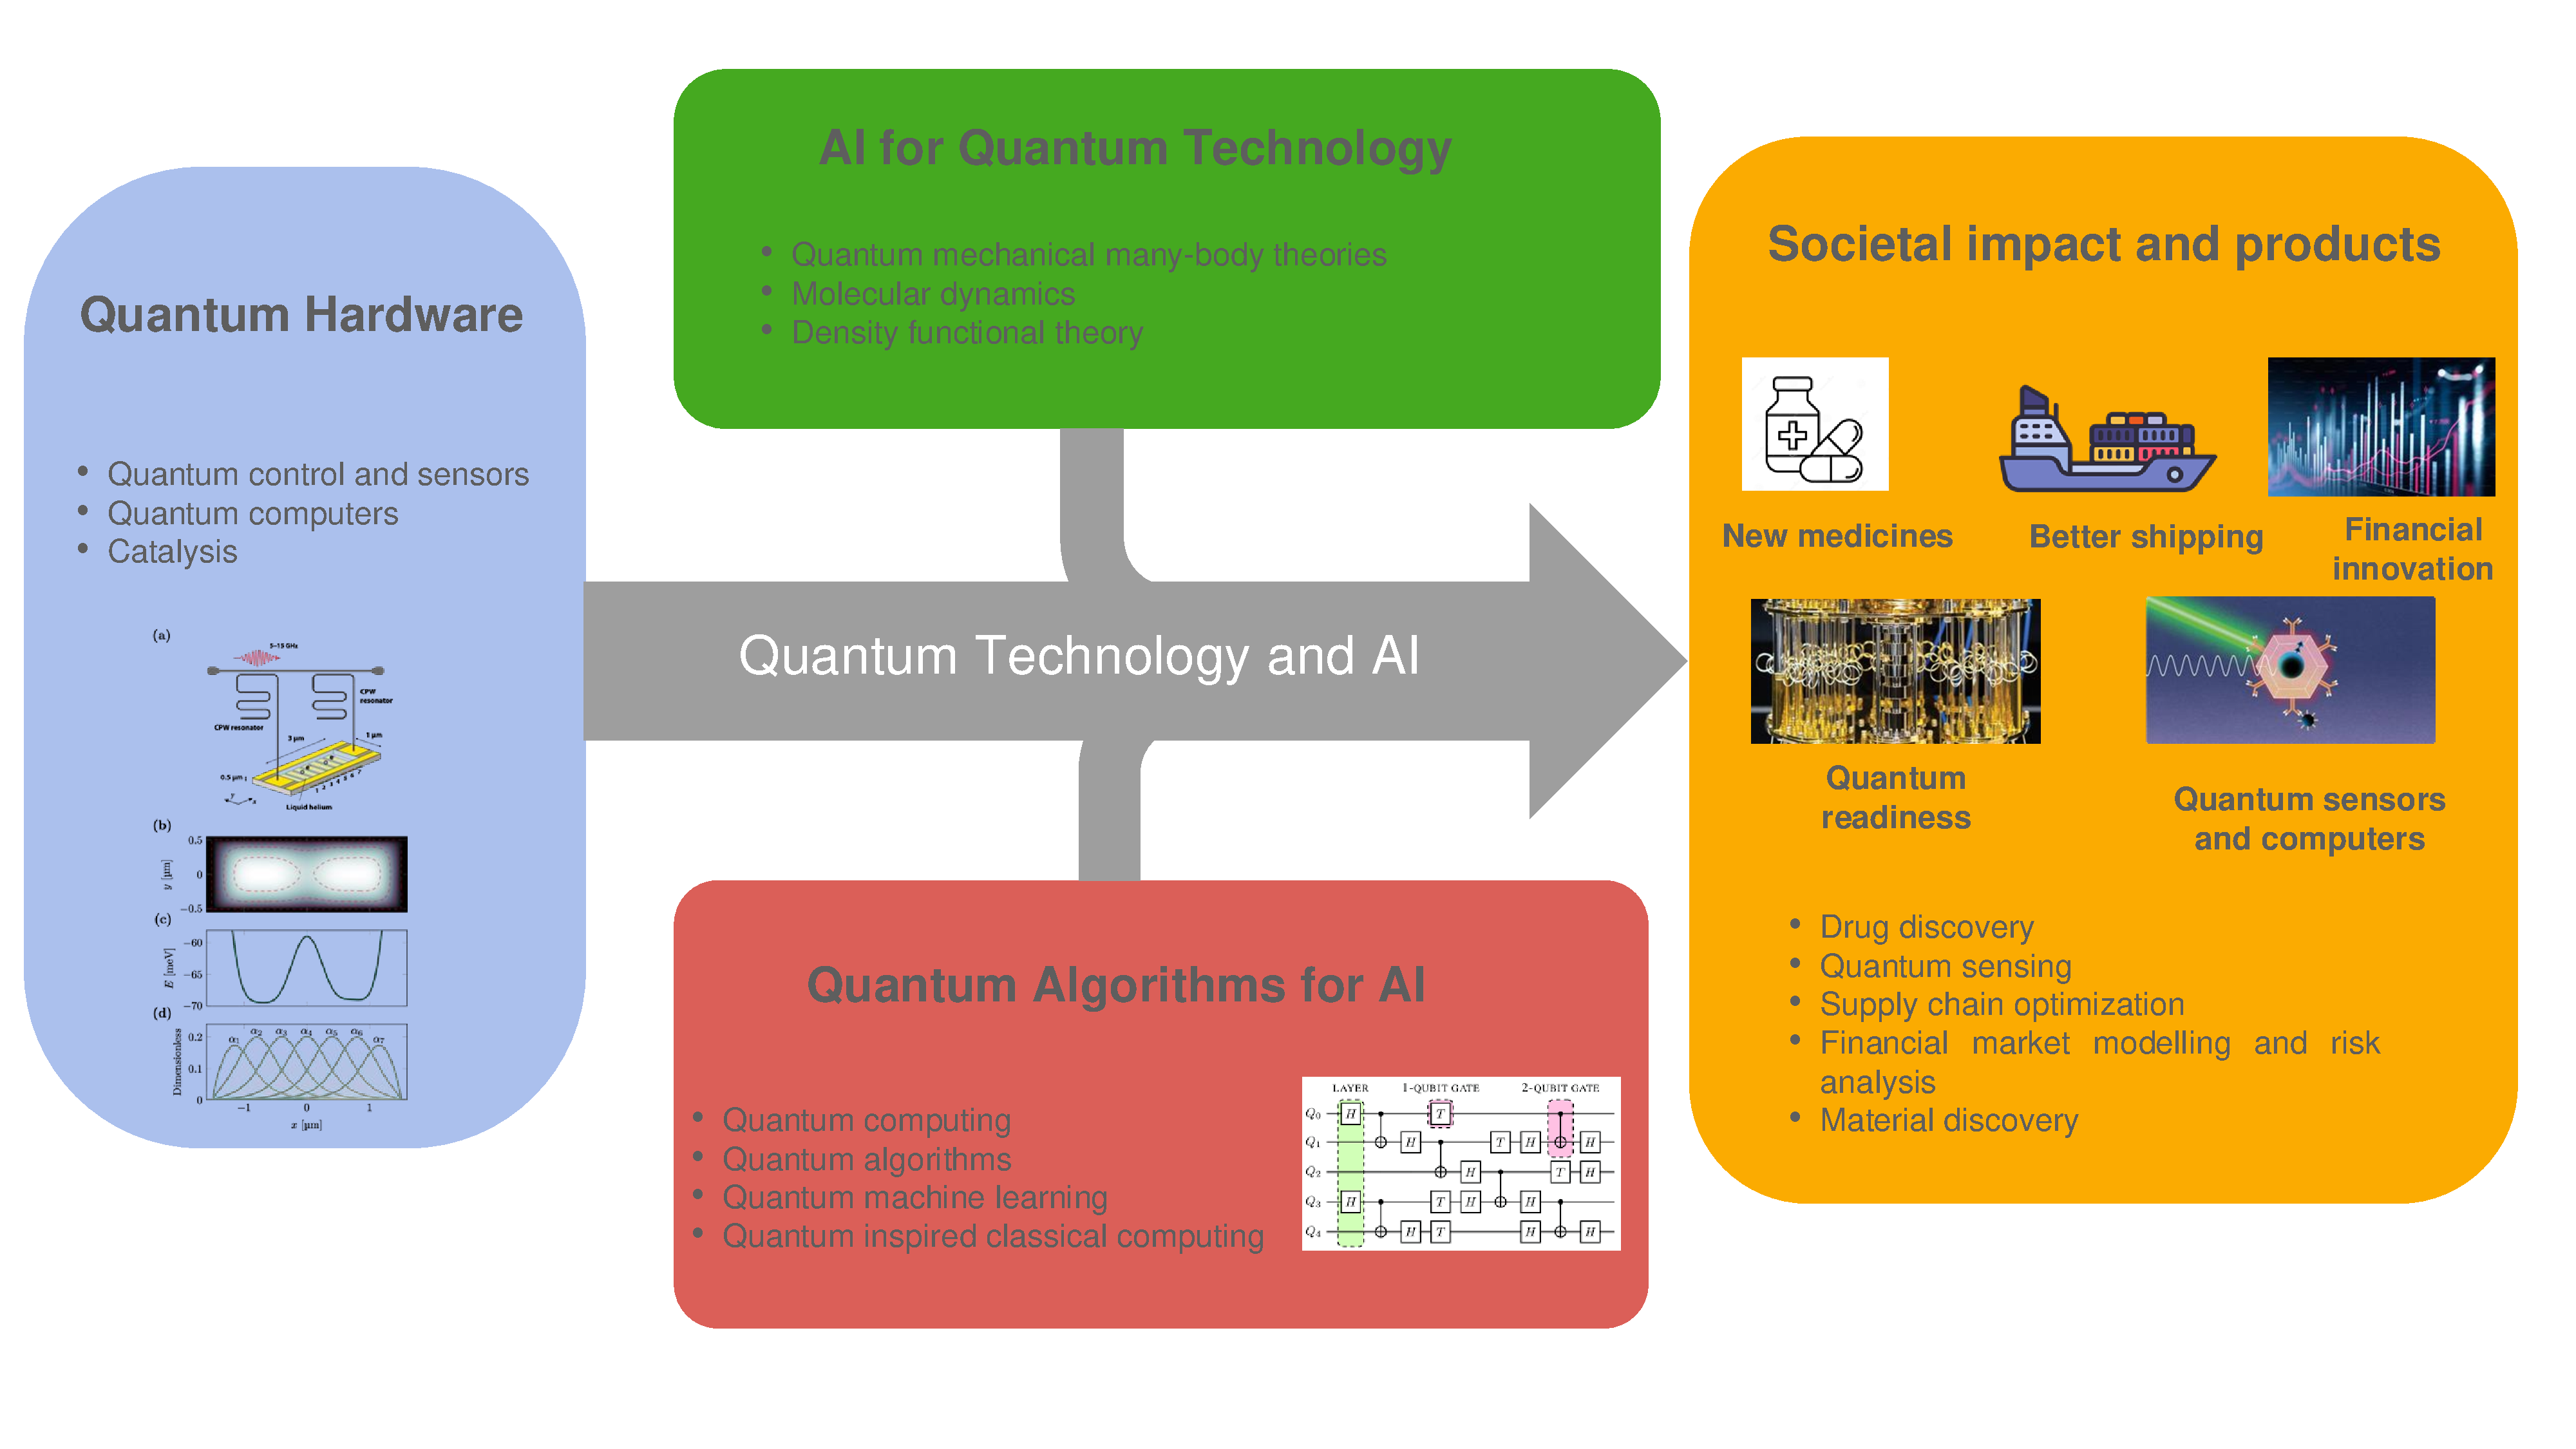
\includegraphics[width=1.05\linewidth]{figures/figureintro.pdf}}

\end{frame}



%-----------------------------------------------------------
\section{Introduction to Machine Learning}
\begin{frame}{What is Machine Learning?}
Machine Learning (ML) is the study of algorithms that improve through data experience.

\textbf{Types of Machine Learning:}
\begin{itemize}
    \item \textbf{Supervised Learning:} Labeled data for classification or regression.
    \item \textbf{Unsupervised Learning:} No labels; discover hidden patterns.
    \item \textbf{Reinforcement Learning:} Learning through interaction with the environment.
\end{itemize}


\textbf{ML Workflow:}
\[
\text{Data} \rightarrow \text{Model Training} \rightarrow \text{Prediction}
\]
\end{frame}



%-----------------------------------------------------------
\section{Introduction to Quantum Computing}
\begin{frame}{What is Quantum Computing?}
Quantum computing leverages principles of quantum mechanics to perform computations beyond classical capabilities.

\vspace{10pt}
\textbf{Key Concepts:}
\begin{itemize}
\item \textbf{Superposition:} Qubits can exist in a combination of states.
\item \textbf{Entanglement:} Correlation between qubits regardless of distance.
\item \textbf{Quantum Interference:} Probability amplitudes interfere to solve problems.
\end{itemize}

\textbf{Qubit Representation:}
\[
\ket{\psi} = \alpha \ket{0} + \beta \ket{1}, \quad |\alpha|^2 + |\beta|^2 = 1
\]
\end{frame}


%-----------------------------------------------------------
\section{Quantum Machine Learning (QML)}
\begin{frame}{What is Quantum Machine Learning?}
\textbf{Quantum Machine Learning (QML)} integrates quantum computing with machine learning algorithms to exploit quantum advantages.

\vspace{10pt}
\textbf{Motivation:}
\begin{itemize}
    \item High-dimensional Hilbert spaces for better feature representation.
    \item Quantum parallelism for faster computation.
    \item Quantum entanglement for richer data encoding.
\end{itemize}


\end{frame}

\section{Quantum Speedups}
\begin{frame}{Quantum Speedups in ML}
\textbf{Why Quantum?}
\begin{itemize}
    \item \textbf{Quantum Parallelism:} Process multiple states simultaneously.
    \item \textbf{Quantum Entanglement:} Correlated states for richer information.
    \item \textbf{Quantum Interference:} Constructive and destructive interference to enhance solutions.
\end{itemize}

\textbf{Example - Grover's Algorithm:}
\[
\text{Quantum Search Complexity: } O(\sqrt{N}) \text{ vs. } O(N)
\]

\textbf{Advantage:}
- Speedups in high-dimensional optimization and linear algebra problems.
\end{frame}

%-----------------------------------------------------------
\section{Challenges in Quantum Machine Learning}
\begin{frame}{Challenges and Limitations}
\textbf{1. Quantum Hardware Limitations:}
\begin{itemize}
    \item Noisy Intermediate-Scale Quantum (NISQ) devices.
    \item Decoherence and limited qubit coherence times.
\end{itemize}

\textbf{2. Data Encoding:}
\begin{itemize}
    \item Efficient embedding of classical data into quantum states.
\end{itemize}

\textbf{3. Scalability:}
\begin{itemize}
    \item Difficult to scale circuits to large datasets.
\end{itemize}
\end{frame}



\begin{frame}[plain,fragile]
\frametitle{AI/ML and some statements you may have heard (and what do they mean?)}



\begin{enumerate}
\item Fei-Fei Li on ImageNet: \textbf{map out the entire world of objects} (\href{{https://cacm.acm.org/news/219702-the-data-that-transformed-ai-research-and-possibly-the-world/fulltext}}{The data that transformed AI research})

\item Russell and Norvig in their popular textbook: \textbf{relevant to any intellectual task; it is truly a universal field} (\href{{http://aima.cs.berkeley.edu/}}{Artificial Intelligence, A modern approach})

\item Woody Bledsoe puts it more bluntly: \textbf{in the long run, AI is the only science} (quoted in Pamilla McCorduck, \href{{https://www.pamelamccorduck.com/machines-who-think}}{Machines who think})
\end{enumerate}

\noindent
If you wish to have a critical read on AI/ML from a societal point of view, see \href{{https://www.katecrawford.net/}}{Kate Crawford's recent text Atlas of AI}.

\textbf{Here: with AI/ML we intend a collection of machine learning methods with an emphasis on statistical learning and data analysis}
\end{frame}






\begin{frame}[plain,fragile]
\frametitle{Machine learning and AI models are computationally expensive}


% inline figure
\centerline{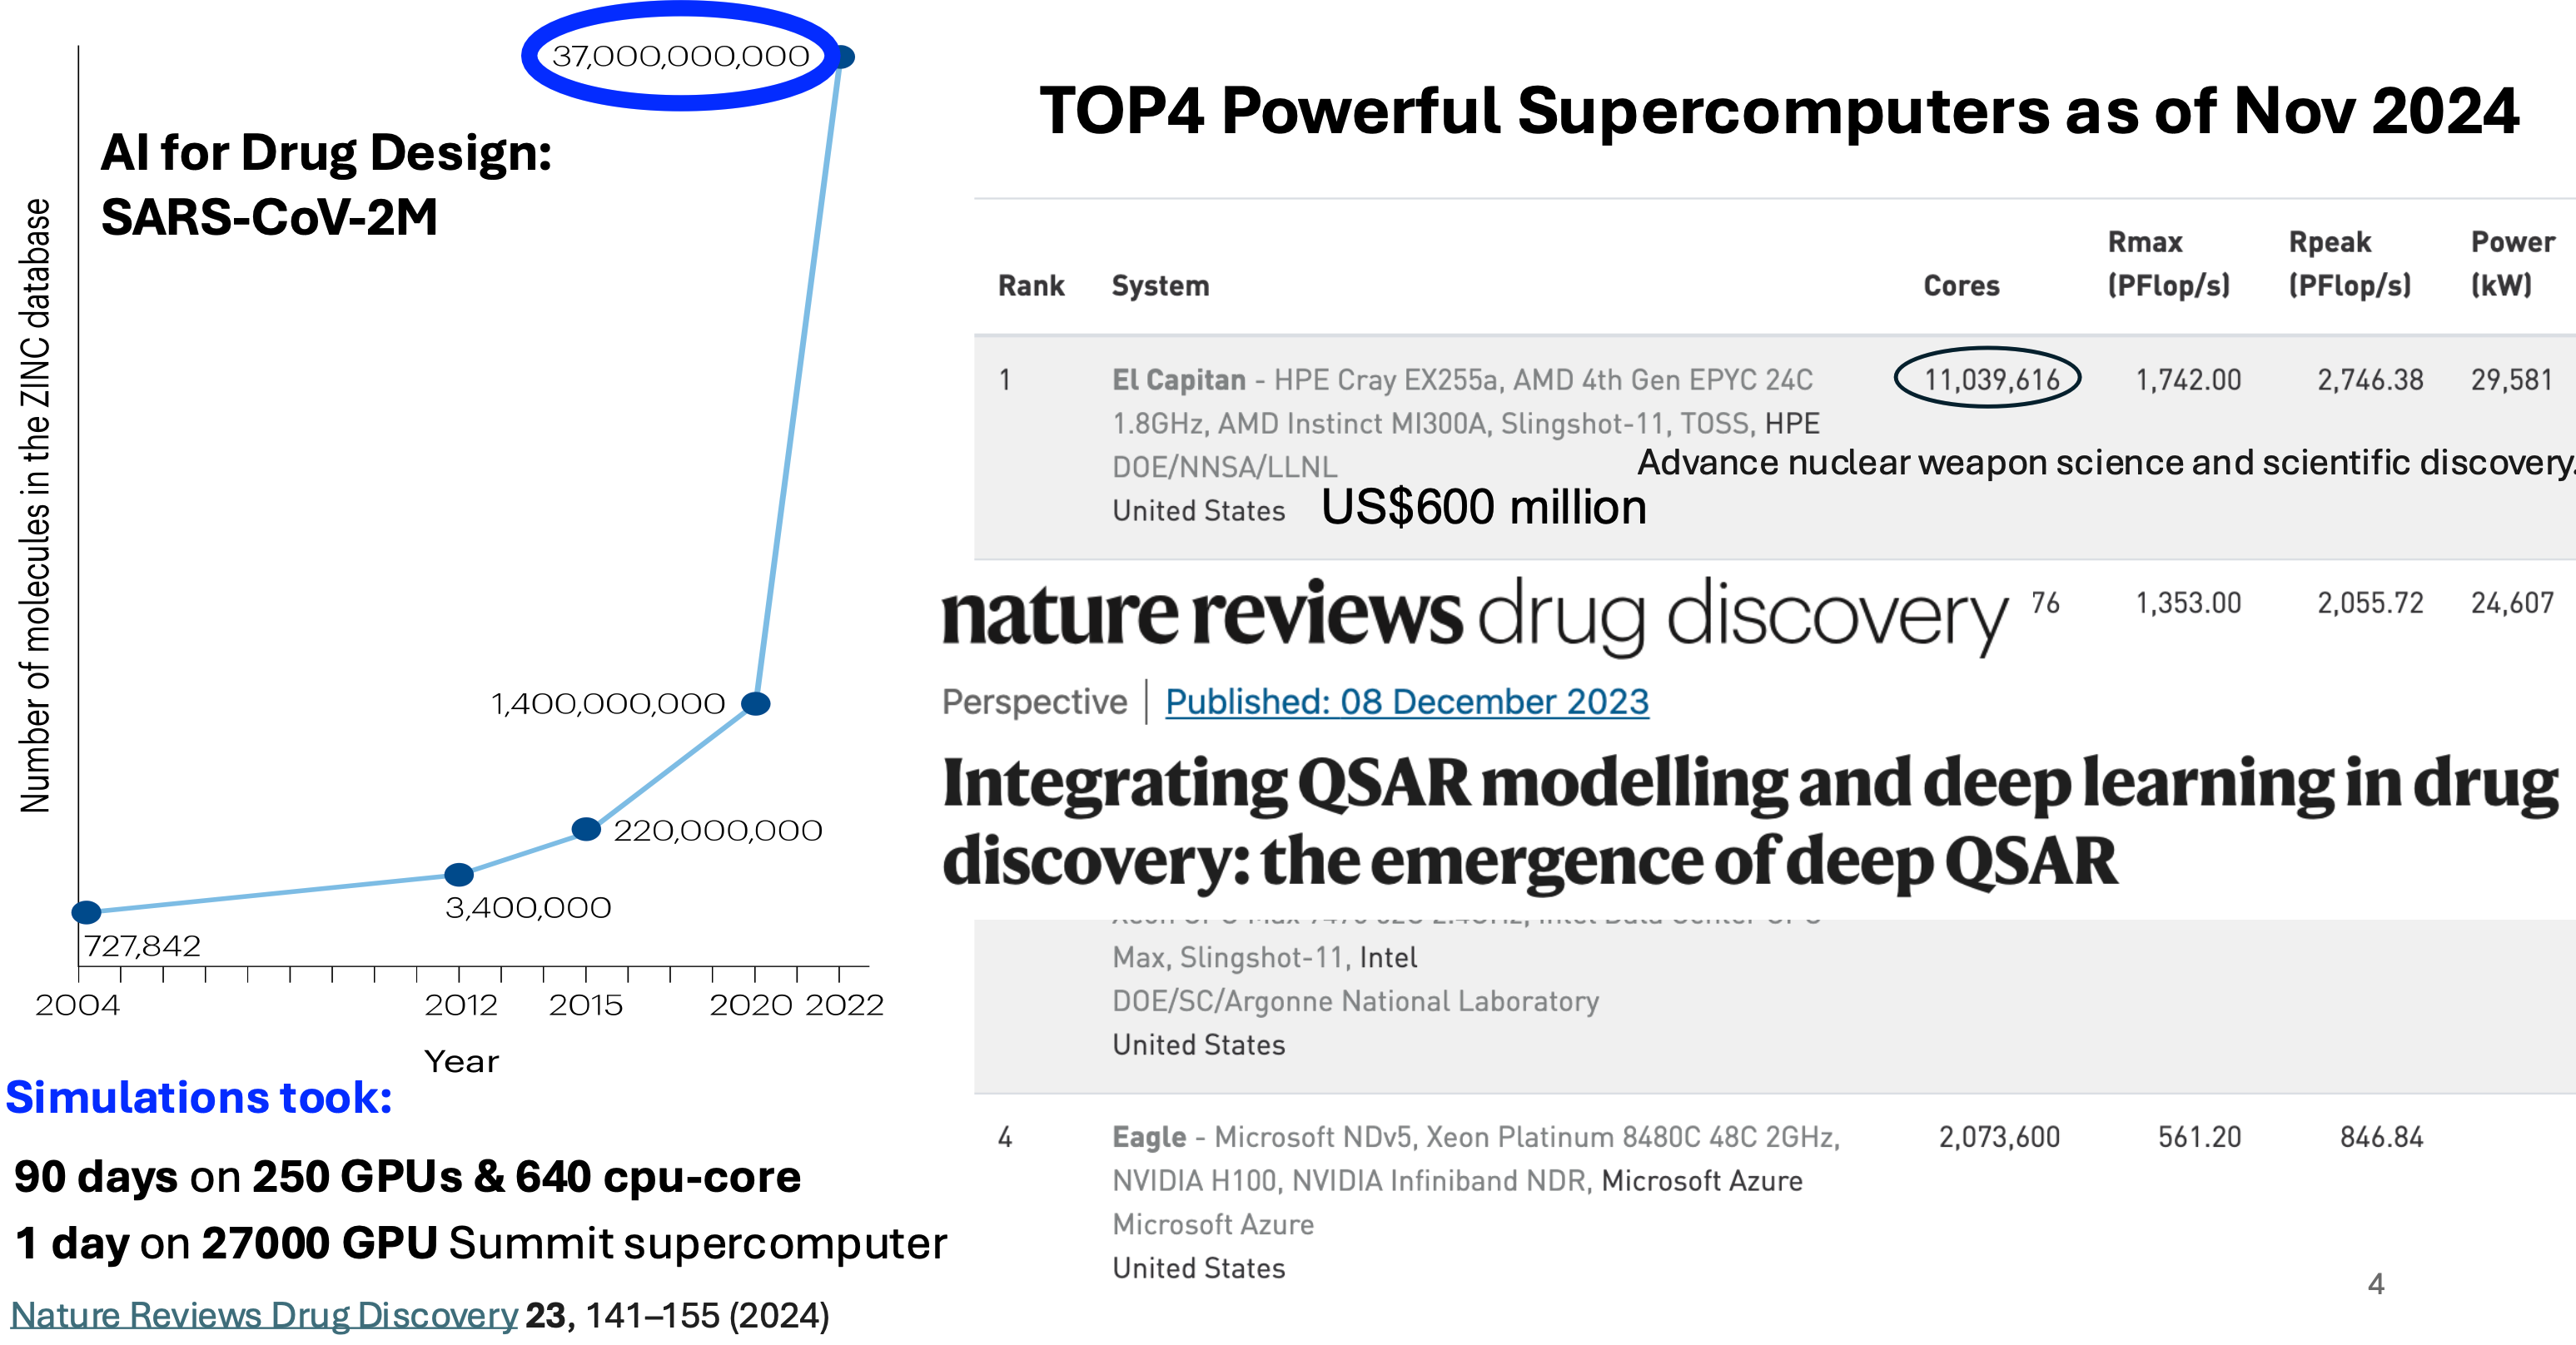
\includegraphics[width=1.0\linewidth]{figures/aitalk2.png}}

\end{frame}


\begin{frame}[plain,fragile]
\frametitle{And power greedy, perhaps quantum computers can reduce the impact?}

% inline figure
\centerline{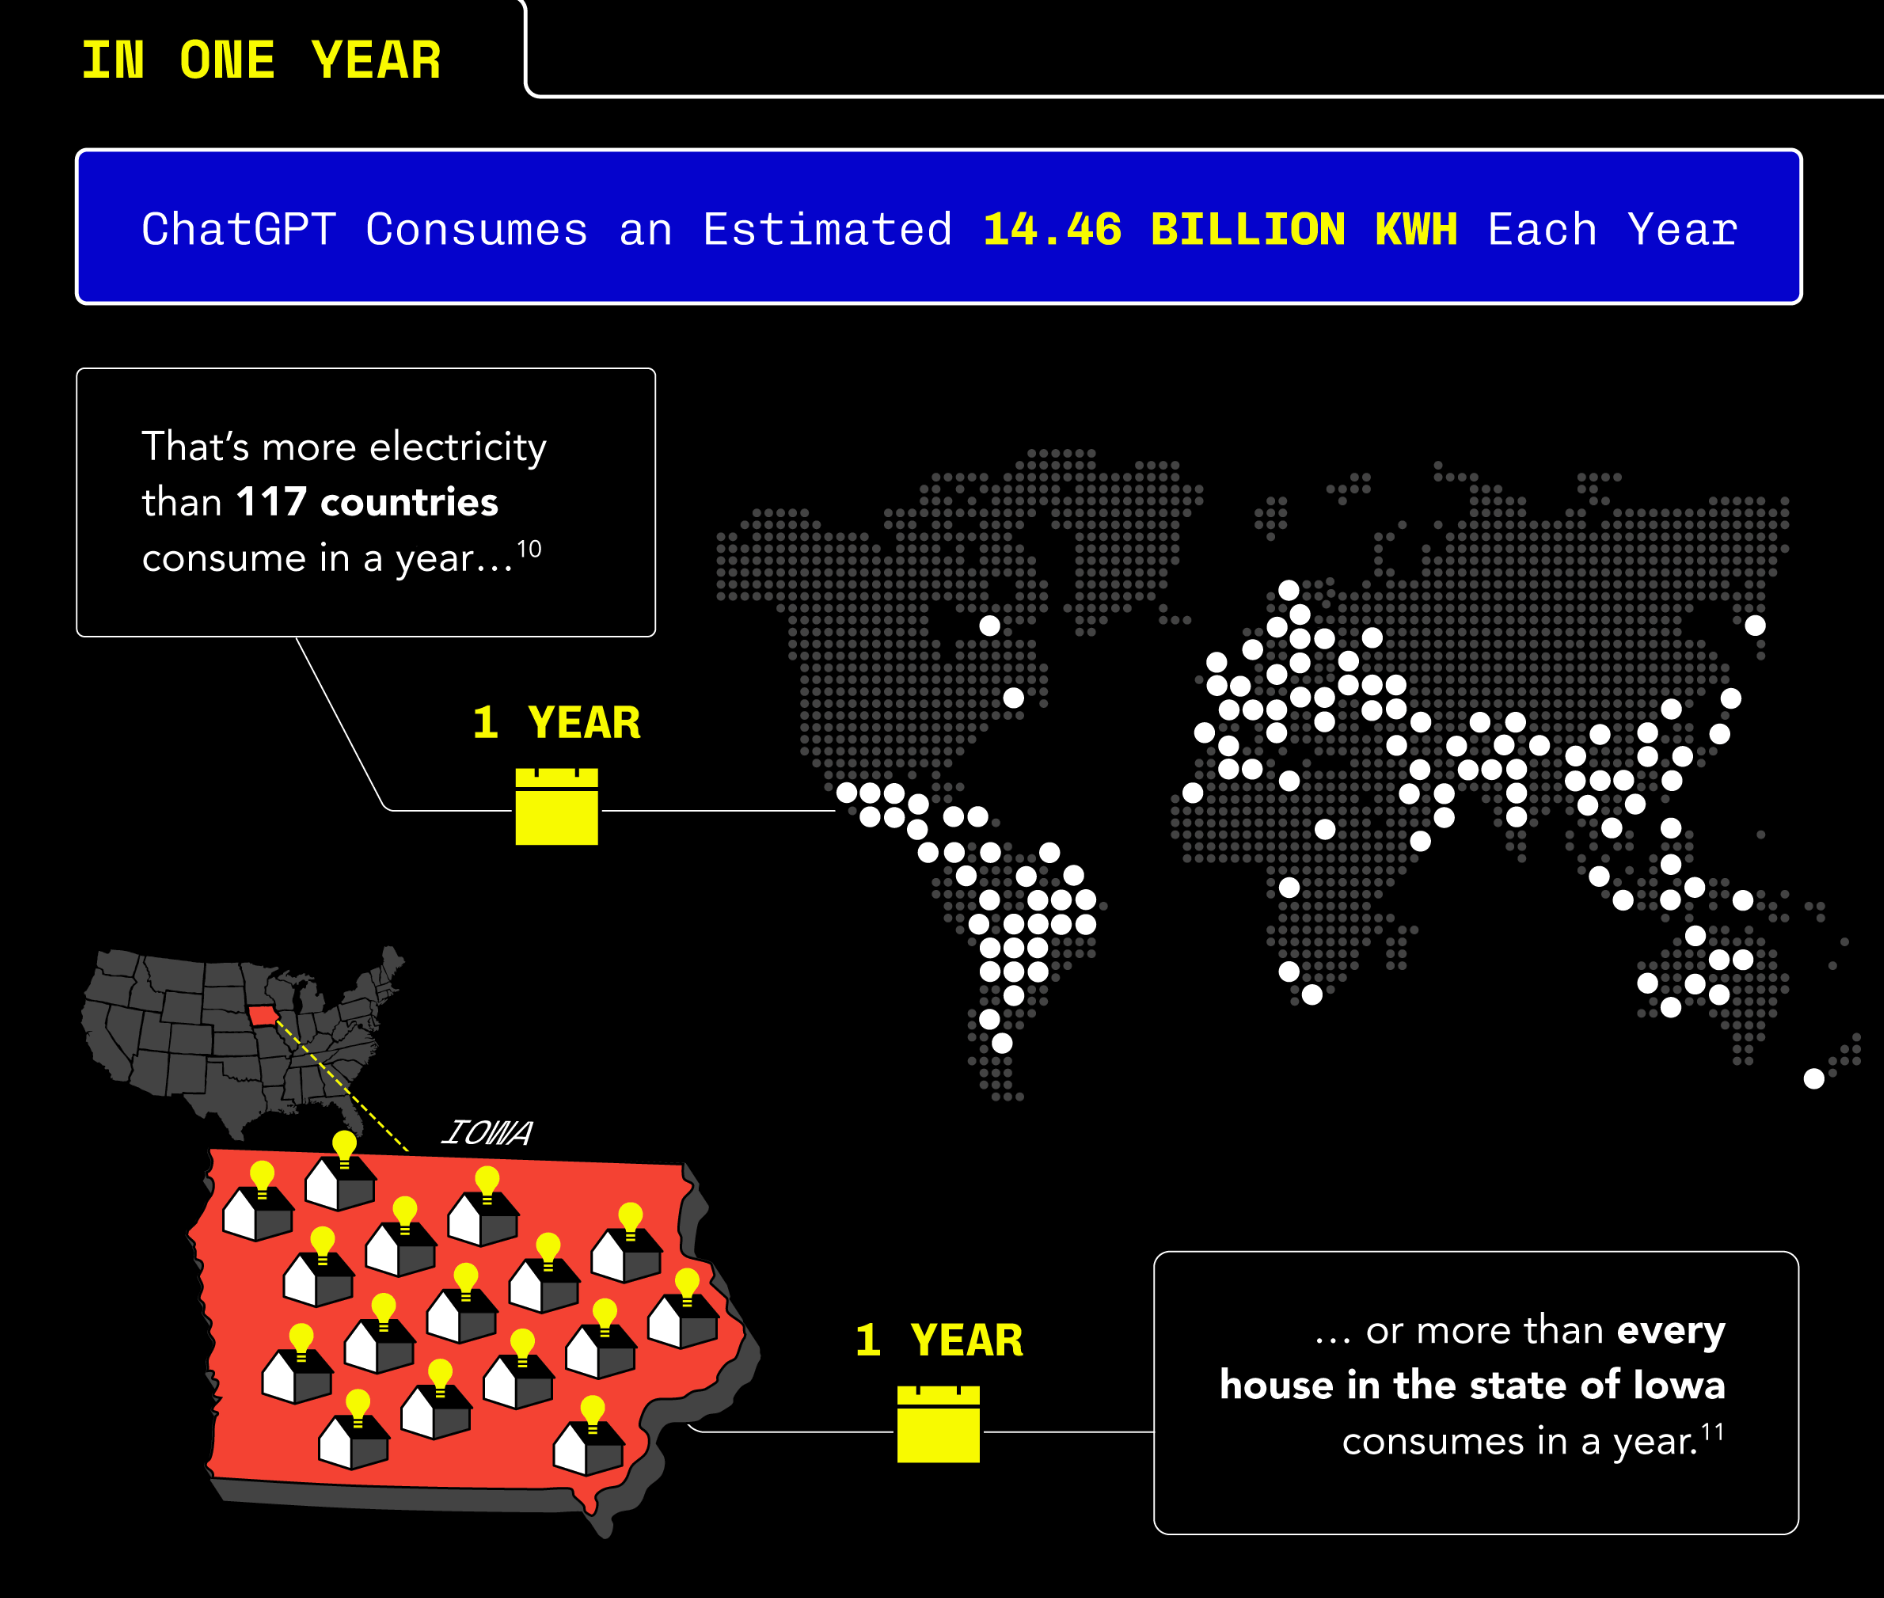
\includegraphics[width=0.7\linewidth]{figures/aitalk1.png}}
Taken from \url{https://www.businessenergyuk.com/knowledge-hub/chatgpt-energy-consumption-visualized/}
\end{frame}



\begin{frame}[plain,fragile]
\frametitle{Main categories of Machine Learning}

\begin{block}{}
Another way to categorize machine learning tasks is to consider the desired output of a system.
Some of the most common tasks are:

\begin{itemize}
  \item Classification: Outputs are divided into two or more classes. The goal is to   produce a model that assigns inputs into one of these classes. An example is to identify  digits based on pictures of hand-written ones. Classification is typically supervised learning.

  \item Regression: Finding a functional relationship between an input data set and a reference data set.   The goal is to construct a function that maps input data to continuous output values.

  \item Clustering: Data are divided into groups with certain common traits, without knowing the different groups beforehand.  It is thus a form of unsupervised learning.
\end{itemize}

\noindent
\end{block}
\end{frame}





\begin{frame}[plain,fragile]
\frametitle{The plethora  of machine learning algorithms/methods}

\begin{enumerate}
\item Deep learning: Neural Networks (NN), Convolutional NN, Recurrent NN, Boltzmann machines, autoencoders and variational autoencoders  and generative adversarial networks, stable diffusion and many more generative models

\item Bayesian statistics and Bayesian Machine Learning, Bayesian experimental design, Bayesian Regression models, Bayesian neural networks, Gaussian processes and much more

\item Dimensionality reduction (Principal component analysis), Clustering Methods and more

\item Ensemble Methods, Random forests, bagging and voting methods, gradient boosting approaches 

\item Linear and logistic regression, Kernel methods, support vector machines and more

\item Reinforcement Learning; Transfer Learning and more 
\end{enumerate}

\noindent
\end{frame}





\begin{frame}[plain,fragile]
\frametitle{Example of discriminative modeling, \href{{https://www.oreilly.com/library/view/generative-deep-learning/9781098134174/ch01.html}}{taken from Generative Deep Learning by David Foster}}

\vspace{6mm}

% inline figure
\centerline{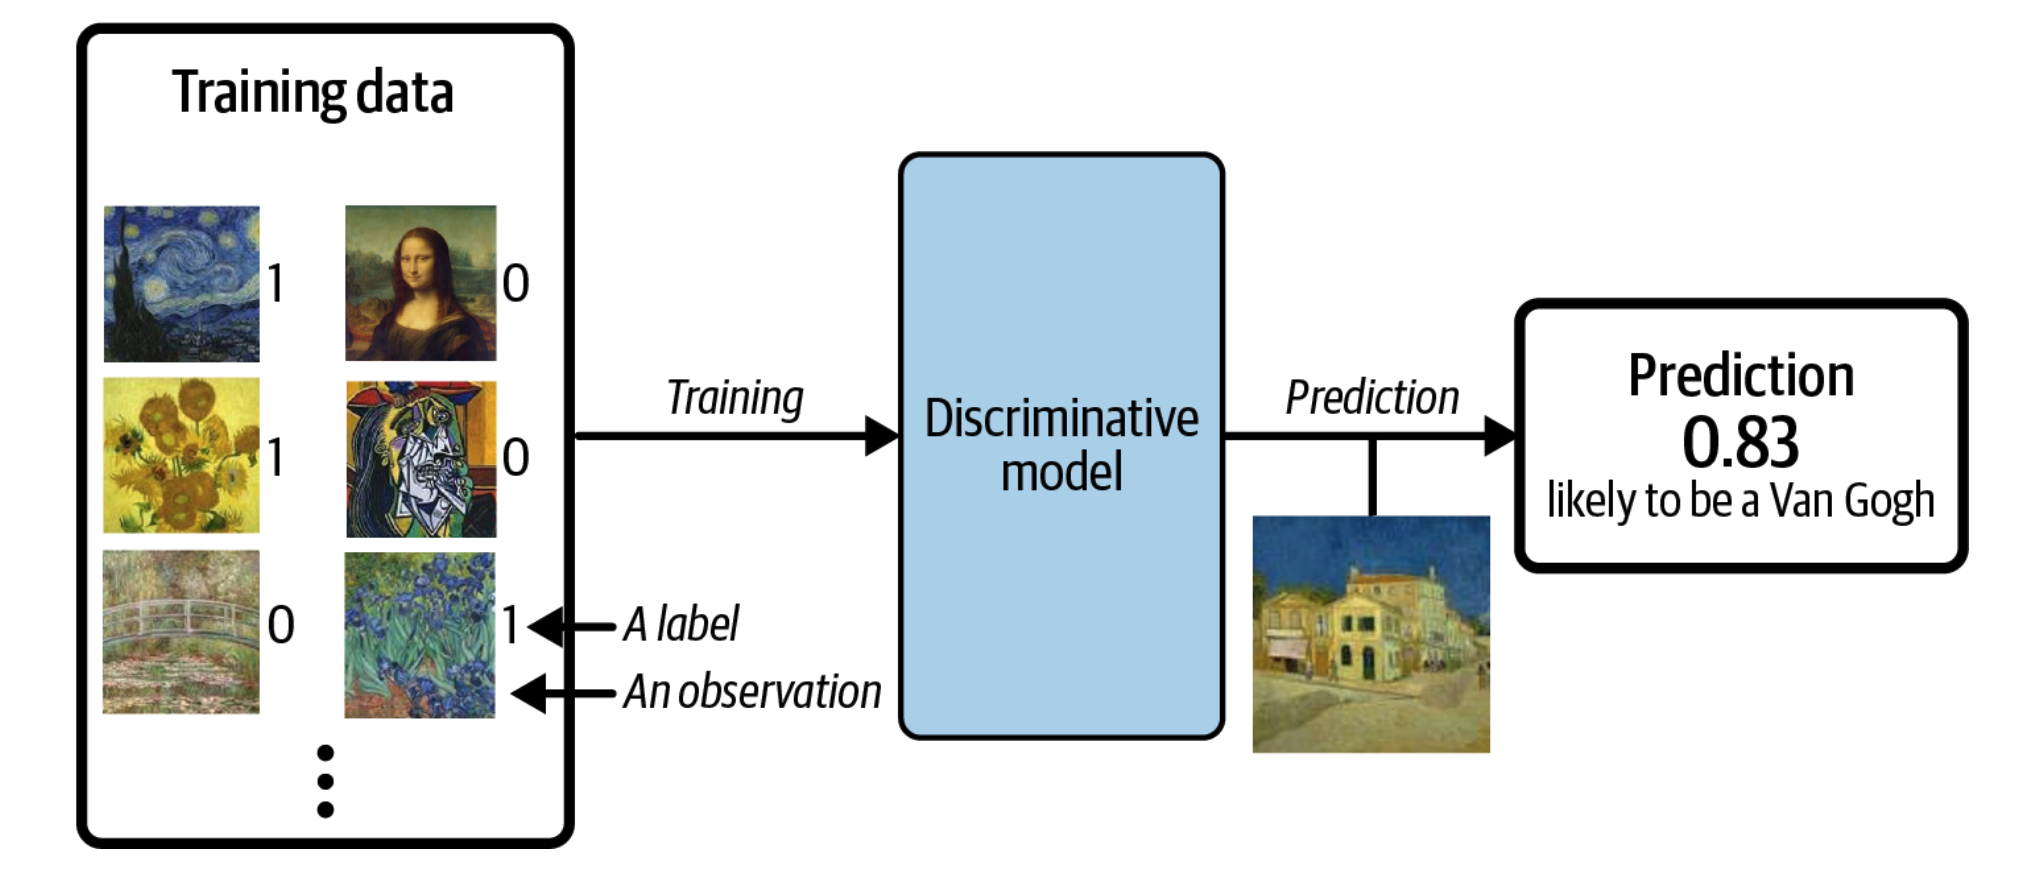
\includegraphics[width=1.0\linewidth]{figures/standarddeeplearning.png}}

\vspace{6mm}
\end{frame}

\begin{frame}[plain,fragile]
\frametitle{Example of generative modeling, \href{{https://www.oreilly.com/library/view/generative-deep-learning/9781098134174/ch01.html}}{taken from Generative Deep Learning by David Foster}}

\vspace{6mm}

% inline figure
\centerline{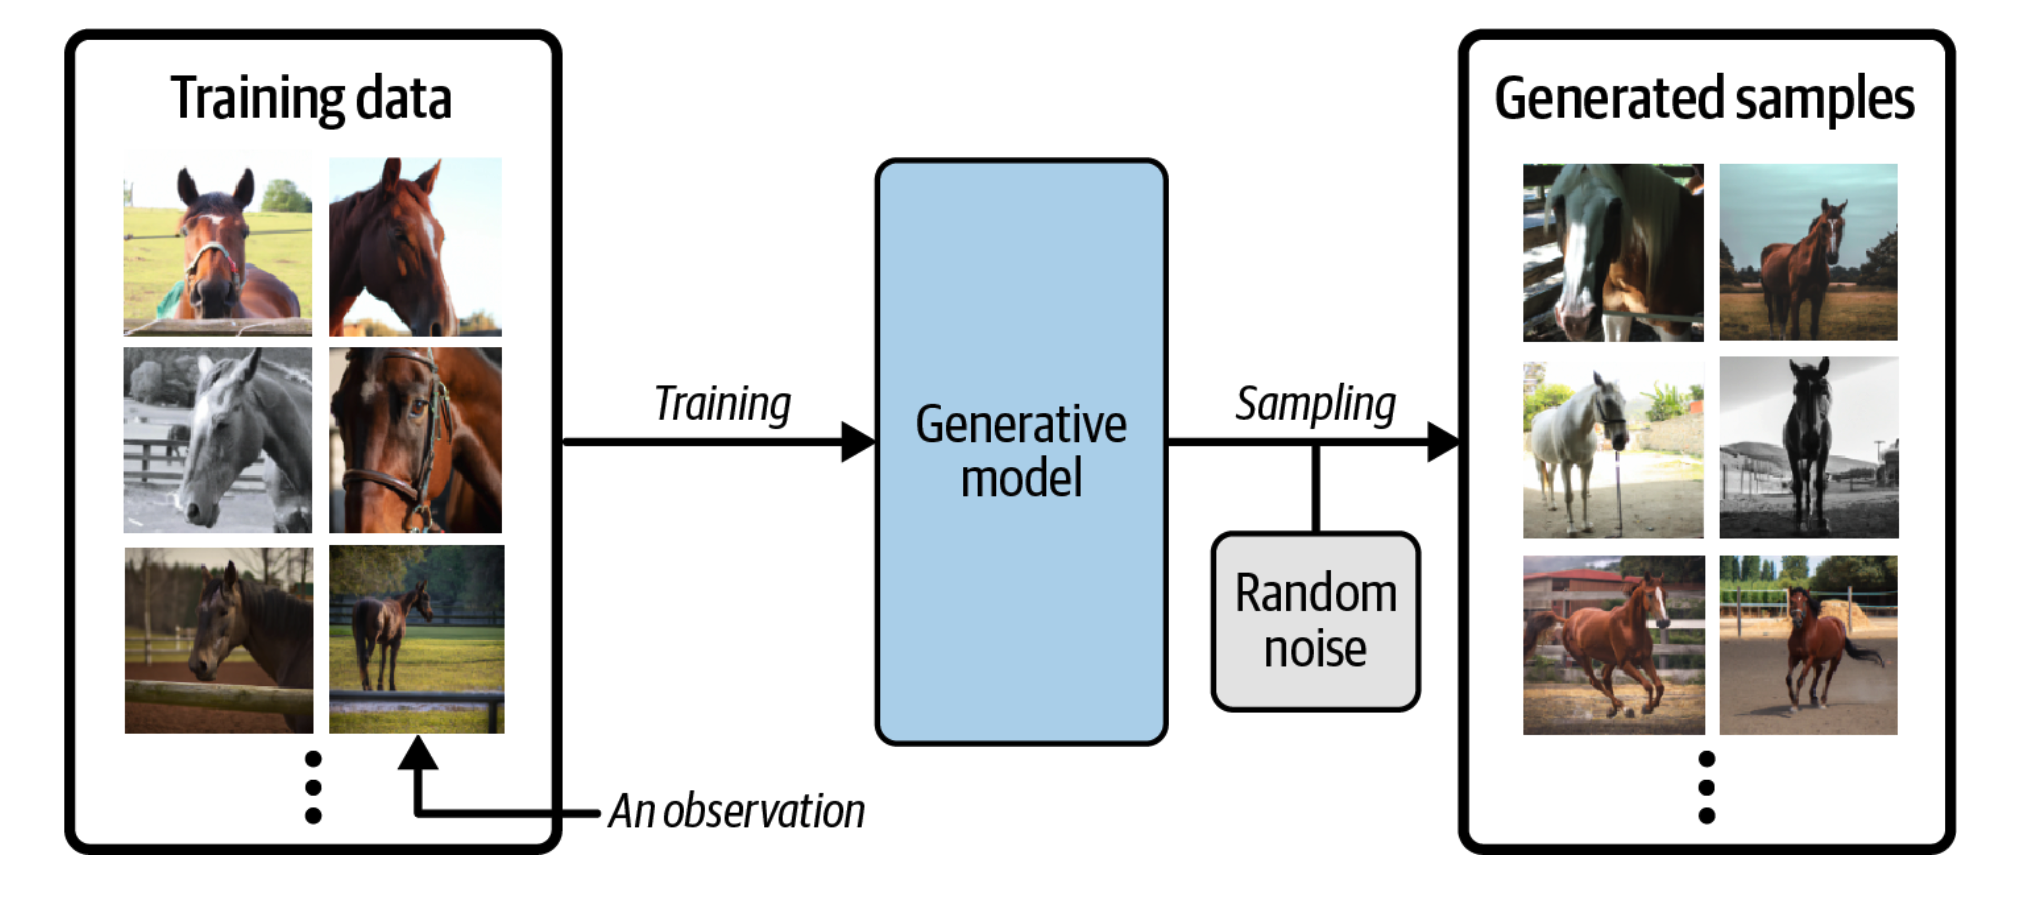
\includegraphics[width=1.0\linewidth]{figures/generativelearning.png}}

\vspace{6mm}
\end{frame}

\begin{frame}[plain,fragile]
\frametitle{Taxonomy of generative deep learning, \href{{https://www.oreilly.com/library/view/generative-deep-learning/9781098134174/ch01.html}}{taken from Generative Deep Learning by David Foster}}

\vspace{6mm}

% inline figure
\centerline{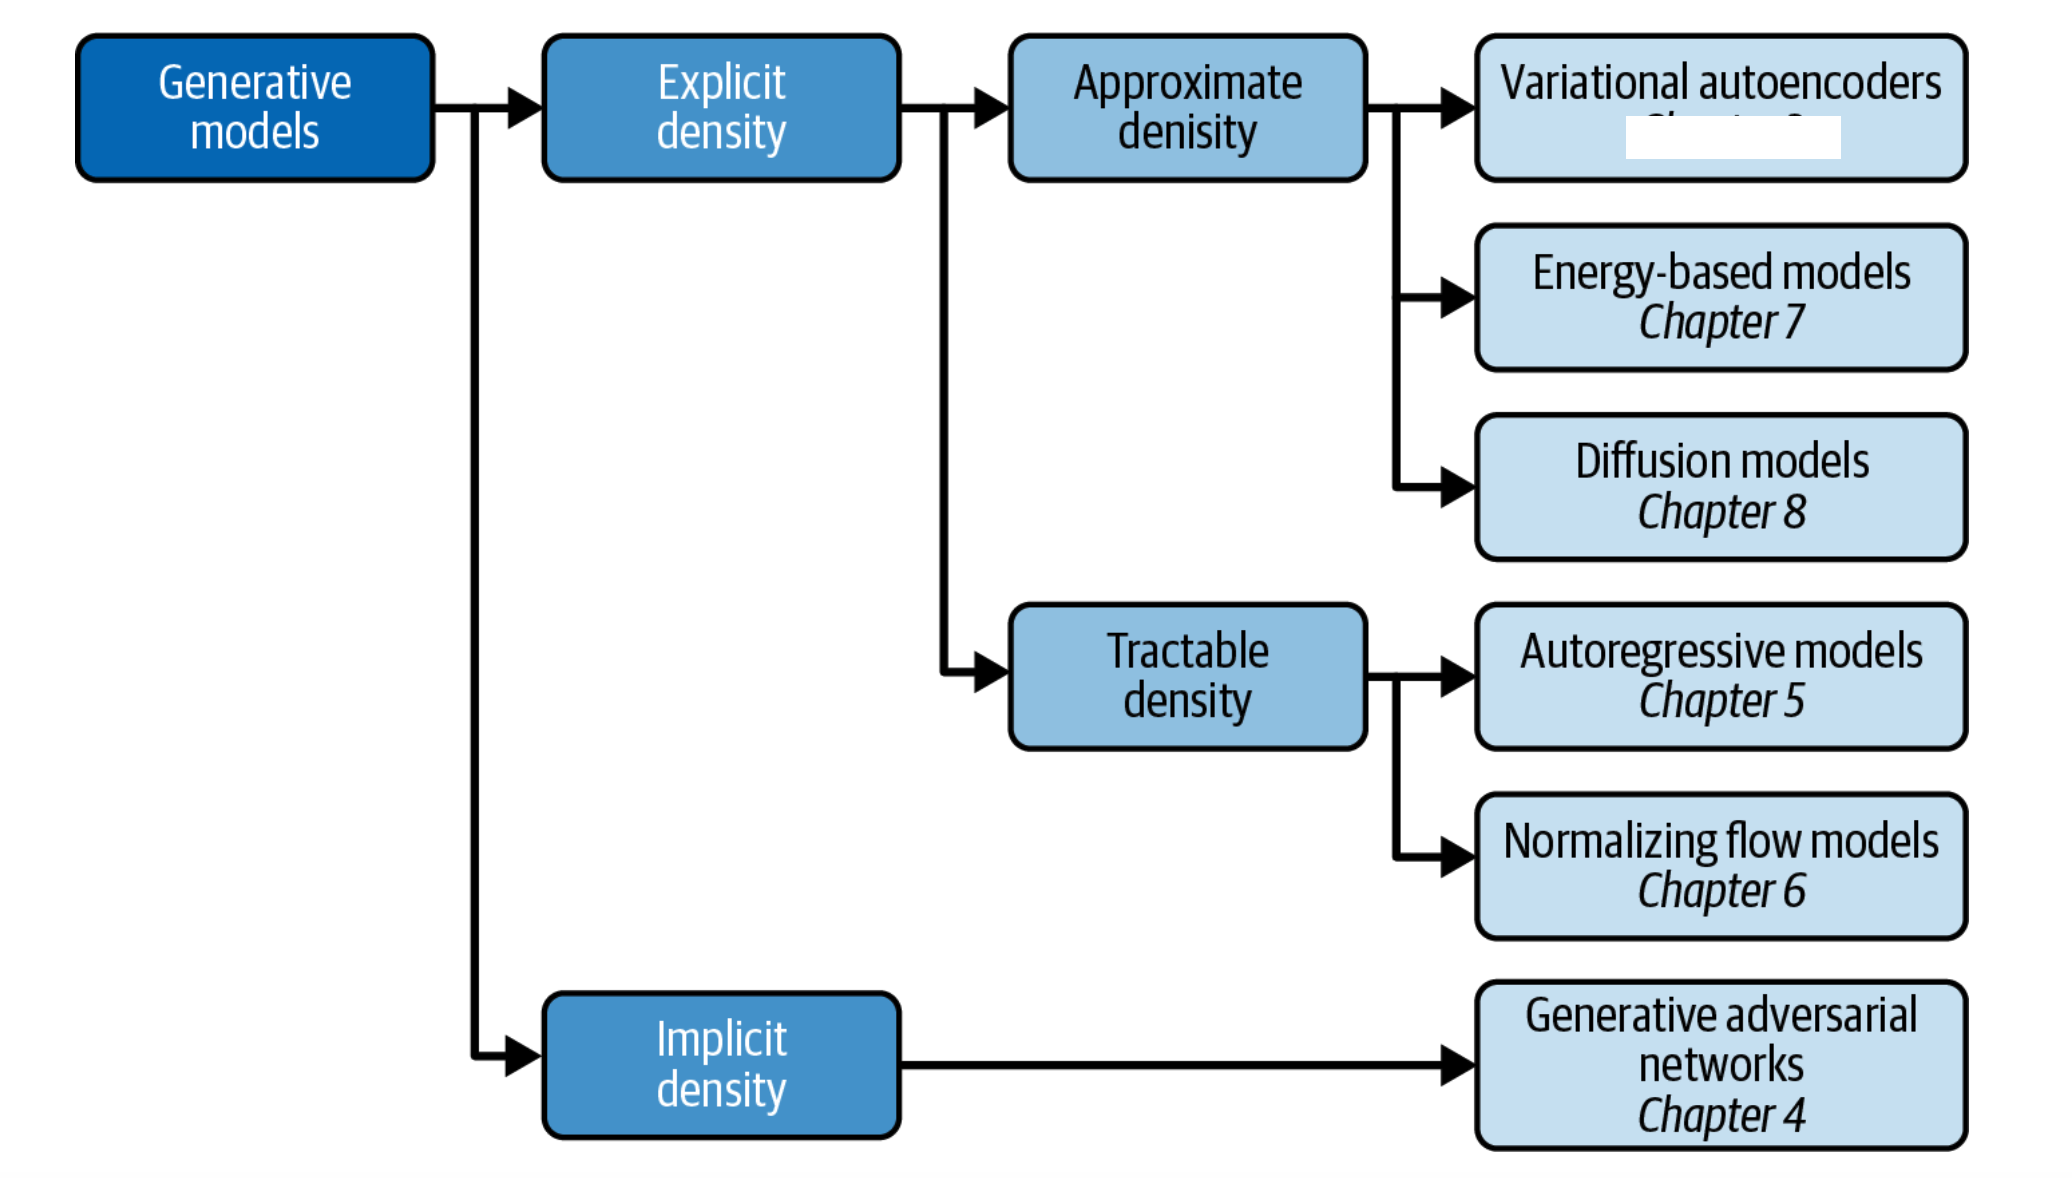
\includegraphics[width=1.0\linewidth]{figures/generativemodels.png}}

\vspace{6mm}
\end{frame}


\begin{frame}[plain,fragile]
\frametitle{What are the basic Machine Learning ingredients?}

\begin{block}{}
Almost every problem in ML and data science starts with the same ingredients:
\begin{itemize}
\item The dataset $\bm{x}$ (could be some observable quantity of the system we are studying)

\item A model which is a function of a set of parameters $\bm{\alpha}$ that relates to the dataset, say a likelihood  function $p(\bm{x}\vert \bm{\alpha})$ or just a simple model $f(\bm{\alpha})$

\item A so-called \textbf{loss/cost/risk} function $\mathcal{C} (\bm{x}, f(\bm{\alpha}))$ which allows us to decide how well our model represents the dataset. 
\end{itemize}

\noindent
We seek to minimize the function $\mathcal{C} (\bm{x}, f(\bm{\alpha}))$ by finding the parameter values which minimize $\mathcal{C}$. This leads to  various minimization algorithms. It may surprise many, but at the heart of all machine learning algortihms there is an optimization problem. 
\end{block}
\end{frame}

\begin{frame}[plain,fragile]
\frametitle{Low-level machine learning, the family of ordinary least squares methods}

Our data which we want to apply a machine learning method on, consist
of a set of inputs $\bm{x}^T=[x_0,x_1,x_2,\dots,x_{n-1}]$ and the
outputs we want to model $\bm{y}^T=[y_0,y_1,y_2,\dots,y_{n-1}]$.
We assume  that the output data can be represented (for a regression case) by a continuous function $f$
through
\[
\bm{y}=f(\bm{x})+\bm{\epsilon}.
\]
\end{frame}

\begin{frame}[plain,fragile]
\frametitle{Setting up the equations}

In linear regression we approximate the unknown function with another
continuous function $\tilde{\bm{y}}(\bm{x})$ which depends linearly on
some unknown parameters
$\bm{\theta}^T=[\theta_0,\theta_1,\theta_2,\dots,\theta_{p-1}]$.

The input data can be organized in terms of a so-called design matrix 
with an approximating function $\bm{\tilde{y}}$ 
\[
\bm{\tilde{y}}= \bm{X}\bm{\theta},
\]
\end{frame}

\begin{frame}[plain,fragile]
\frametitle{The objective/cost/loss function}

The  simplest approach is the mean squared error
\[
C(\bm{\Theta})=\frac{1}{n}\sum_{i=0}^{n-1}\left(y_i-\tilde{y}_i\right)^2=\frac{1}{n}\left\{\left(\bm{y}-\bm{\tilde{y}}\right)^T\left(\bm{y}-\bm{\tilde{y}}\right)\right\},
\]
or using the matrix $\bm{X}$ and in a more compact matrix-vector notation as
\[
C(\bm{\Theta})=\frac{1}{n}\left\{\left(\bm{y}-\bm{X}\bm{\theta}\right)^T\left(\bm{y}-\bm{X}\bm{\theta}\right)\right\}.
\]
This function represents one of many possible ways to define the so-called cost function.
\end{frame}

\begin{frame}[plain,fragile]
\frametitle{Training solution}

Optimizing with respect to the unknown parameters $\theta_j$ we get 
\[
\bm{X}^T\bm{y} = \bm{X}^T\bm{X}\bm{\theta},  
\]
and if the matrix $\bm{X}^T\bm{X}$ is invertible we have the optimal values
\[
\hat{\bm{\theta}} =\left(\bm{X}^T\bm{X}\right)^{-1}\bm{X}^T\bm{y}.
\]

We say we 'learn' the unknown parameters $\bm{\theta}$ from the last equation.
\end{frame}


\begin{frame}[plain,fragile]
\frametitle{Why Neural Networks and deep learning?}
\begin{block}{}
According to the \emph{Universal approximation theorem}, a feed-forward
neural network with just a single hidden layer containing a finite
number of neurons can approximate a continuous multidimensional
function to arbitrary accuracy, assuming the activation function for
the hidden layer is a \textbf{non-constant, bounded and
monotonically-increasing continuous function}.
\end{block}
\begin{block}{}
\textbf{You can think of a neural network as a universal approximator}
\end{block}
\end{frame}


\begin{frame}[plain,fragile]
\frametitle{Schematic view on Machine Learning approaches}


% inline figure
\centerline{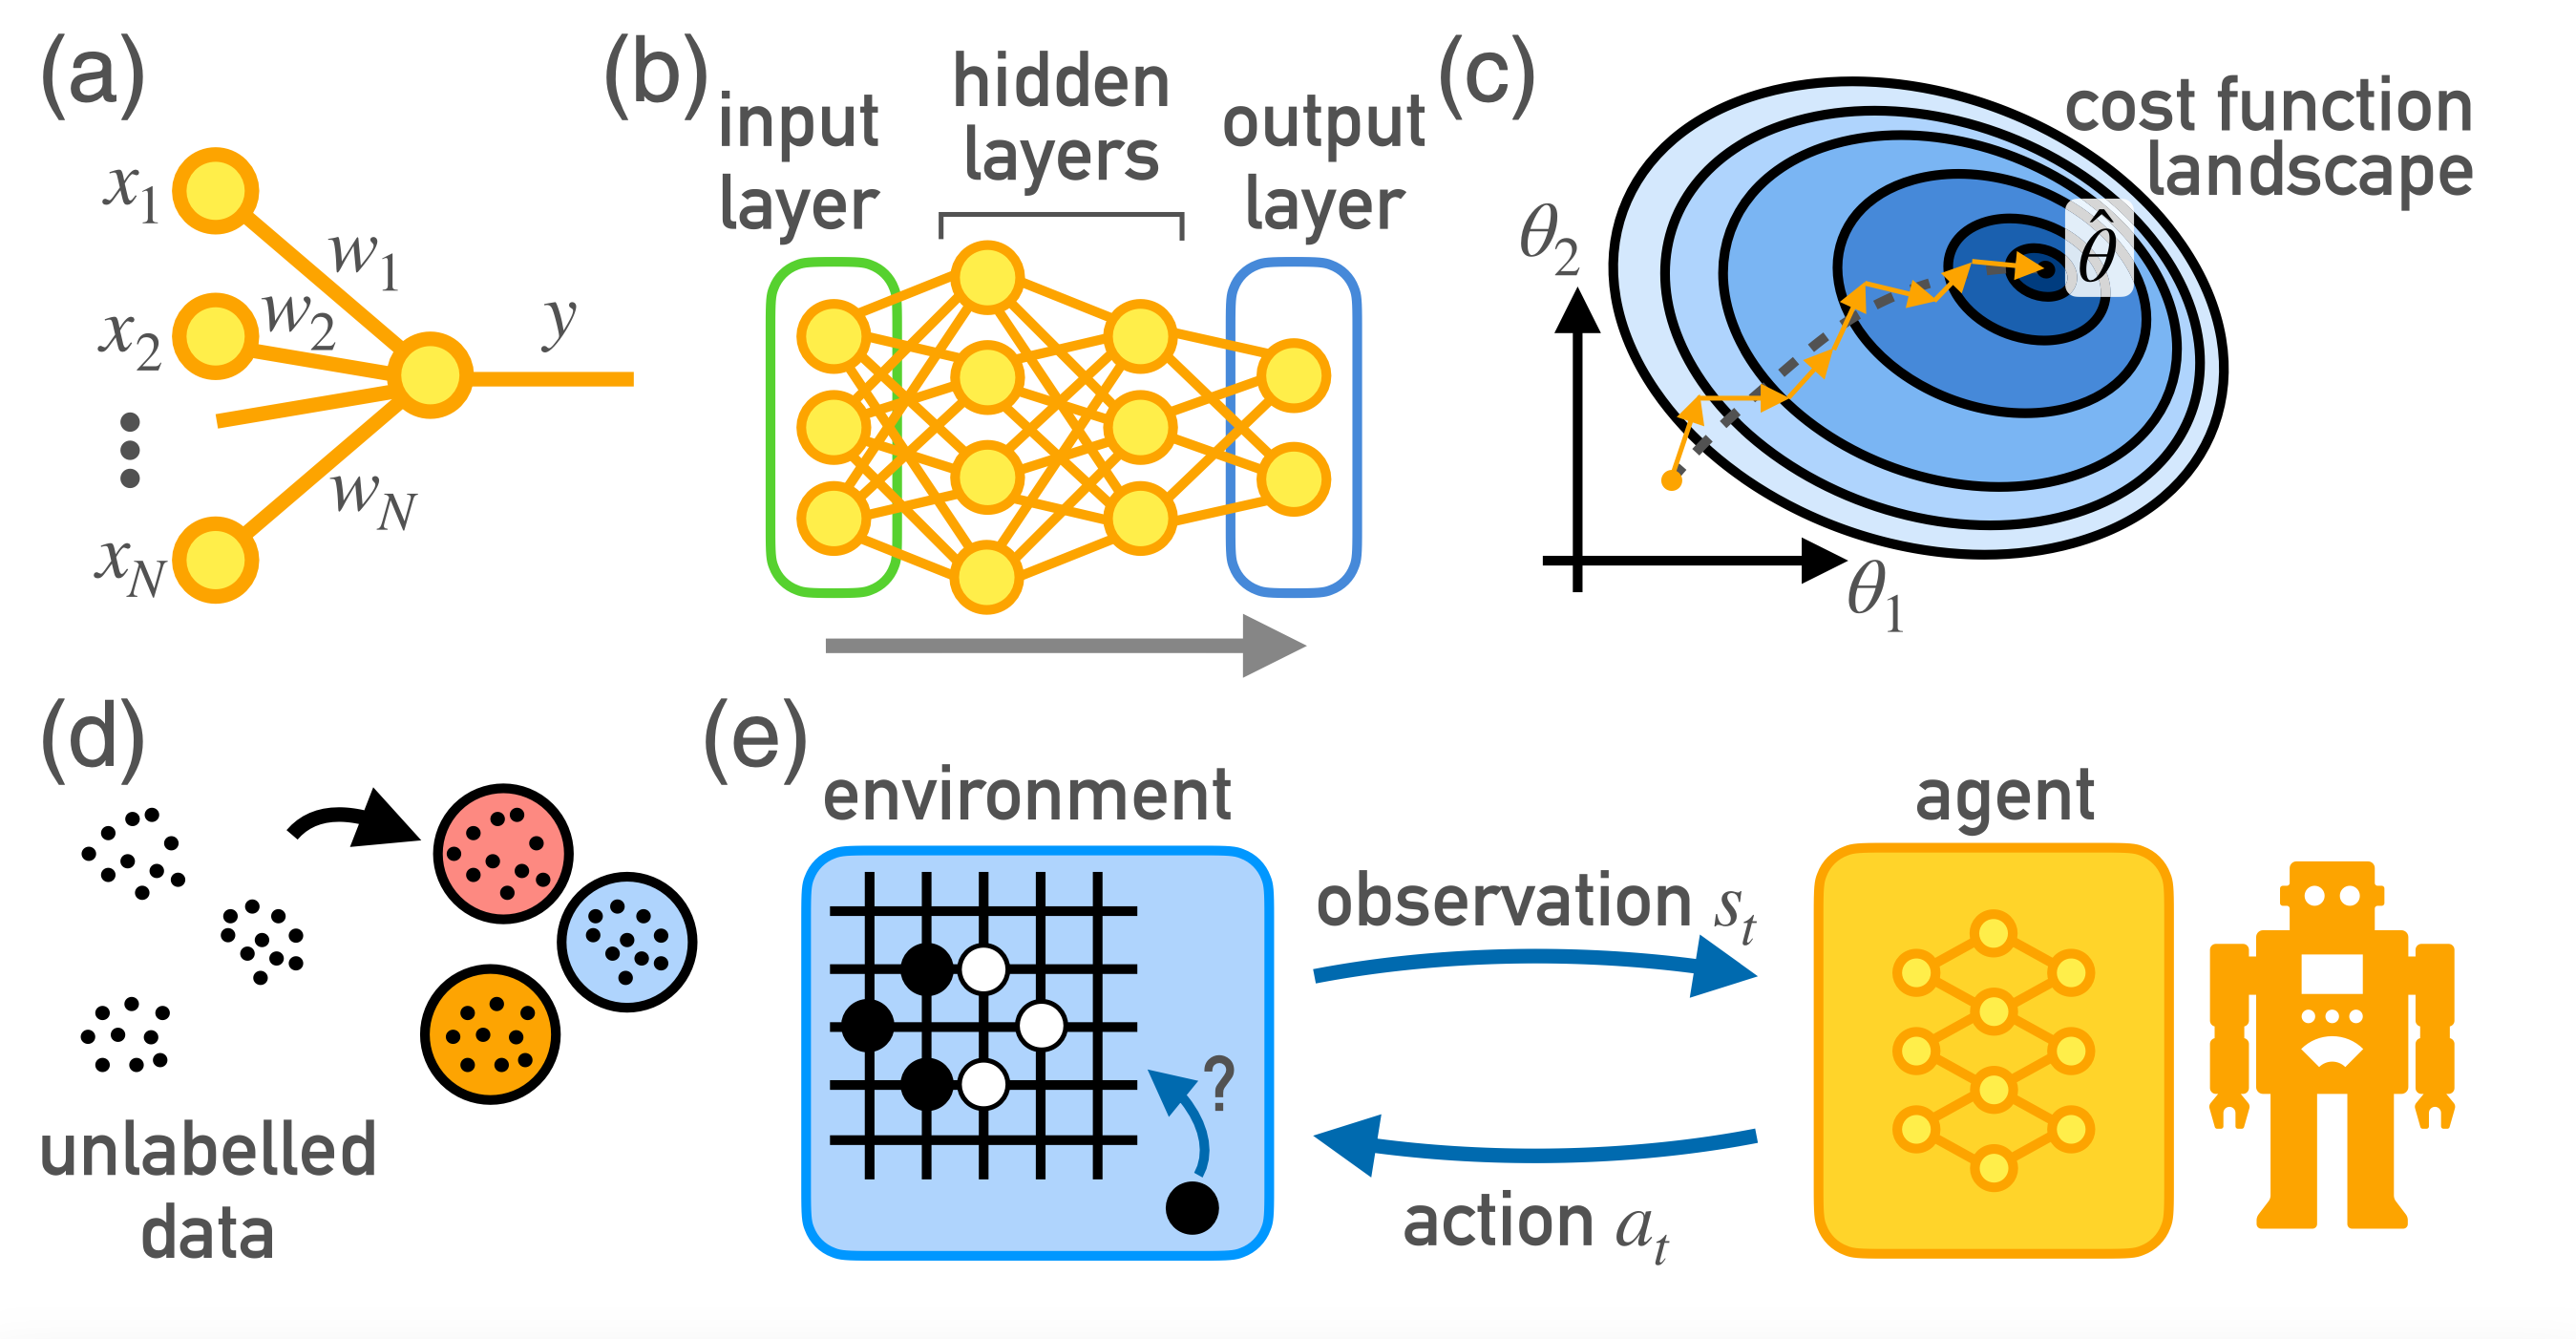
\includegraphics[width=1.05\linewidth]{figures/krenn2}}

\end{frame}




\begin{frame}[plain,fragile]
\frametitle{Scientific Machine Learning}

An important and emerging field is what has been dubbed as scientific ML, see the article by Deiana et al, Applications and Techniques for Fast Machine Learning in Science, Big Data \textbf{5}, 787421 (2022) \href{{https://doi.org/10.3389/fdata.2022.787421}}{\nolinkurl{https://doi.org/10.3389/fdata.2022.787421}}

\begin{block}{}
The authors discuss applications and techniques for fast machine
learning (ML) in science -- the concept of integrating power ML
methods into the real-time experimental data processing loop to
accelerate scientific discovery. The report covers three main areas

\begin{enumerate}
\item applications for fast ML across a number of scientific domains;

\item techniques for training and implementing performant and resource-efficient ML algorithms;

\item and computing architectures, platforms, and technologies for deploying these algorithms.
\end{enumerate}

\noindent
\end{block}
\end{frame}

\begin{frame}[plain,fragile]
\frametitle{ML for detectors}

\vspace{6mm}

% inline figure
\centerline{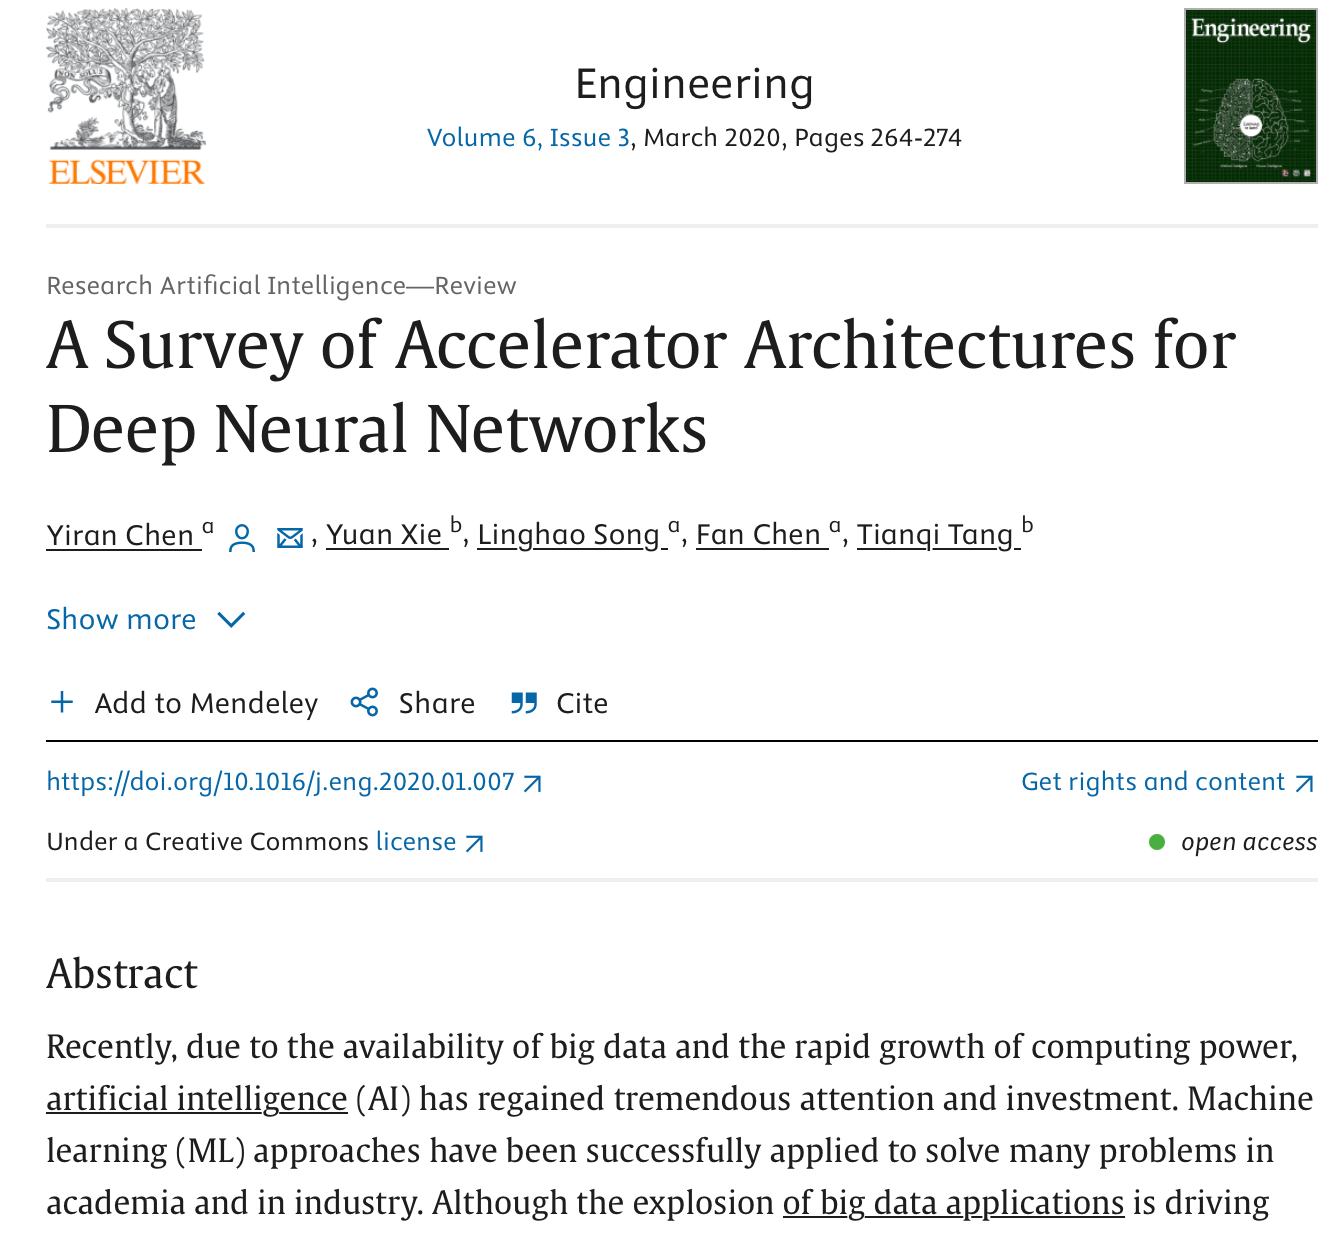
\includegraphics[width=1.0\linewidth]{figures/detectors.png}}

\vspace{6mm}
\end{frame}


\begin{frame}[plain,fragile]
\frametitle{Physics driven Machine Learning}

Another hot topic is what has loosely been dubbed \textbf{Physics-driven deep learning}. See the recent work on \href{{https://www.nature.com/articles/s42256-021-00302-5}}{Learning nonlinear operators via DeepONet based on the universal approximation theorem of operators, Nature Machine Learning, vol 3, 218 (2021)}.

\end{frame}

\begin{frame}[plain,fragile]
\frametitle{And more}

\begin{block}{}
\begin{itemize}
\item An important application of AI/ML methods is to improve the estimation of bias or uncertainty due to the introduction of or lack of physical constraints in various theoretical models.

\item We expect to use AI/ML algorithms and methods to improve our knowledge about  correlations of physical model parameters in data for complex systems. Deep learning methods show great promise in circumventing the exploding dimensionalities encountered in many problems.

\end{itemize}

\noindent
\end{block}
\end{frame}

\begin{frame}[plain,fragile]
\frametitle{Argon-46 by Solli et al., NIMA 1010, 165461 (2021)}

\begin{block}{}
Each row is one event in two projections,
where the color intensity of each point indicates higher charge values
recorded by the detector. The bottom row illustrates a carbon event with
a large fraction of noise, while the top row shows a proton event
almost free of noise. 
\end{block}

% inline figure
\centerline{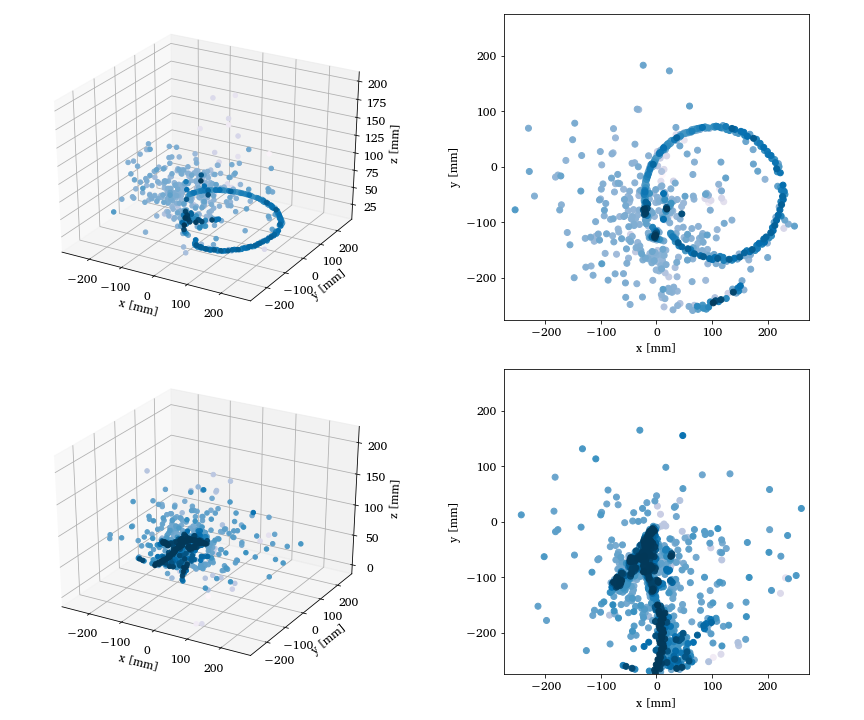
\includegraphics[width=0.6\linewidth]{figures/examples_raw.png}}
\end{frame}



\begin{frame}[plain,fragile]
\frametitle{Many-body physics, Quantum Monte Carlo and deep learning}

\begin{block}{}
Given a Hamiltonian $H$ and a trial wave function $\Psi_T$, the variational principle states that the expectation value of $\langle H \rangle$, defined through 
\[
   \langle E \rangle =
   \frac{\int d\bm{R}\Psi^{\ast}_T(\bm{R})H(\bm{R})\Psi_T(\bm{R})}
        {\int d\bm{R}\Psi^{\ast}_T(\bm{R})\Psi_T(\bm{R})},
\]
is an upper bound to the ground state energy $E_0$ of the hamiltonian $H$, that is 
\[
    E_0 \le \langle E \rangle.
\]
In general, the integrals involved in the calculation of various  expectation values  are multi-dimensional ones. Traditional integration methods such as the Gauss-Legendre will not be adequate for say the  computation of the energy of a many-body system.  \textbf{Basic philosophy: Let a neural network find the optimal wave function}
\end{block}
\end{frame}





\begin{frame}[plain,fragile]
\frametitle{\href{{https://journals.aps.org/prresearch/pdf/10.1103/PhysRevResearch.5.033062}}{Dilute neutron star matter from neural-network quantum states by Fore {\em et al.}, Physical Review Research 5, 033062 (2023)} at density $\rho=0.04$ fm$^{-3}$}

\centerline{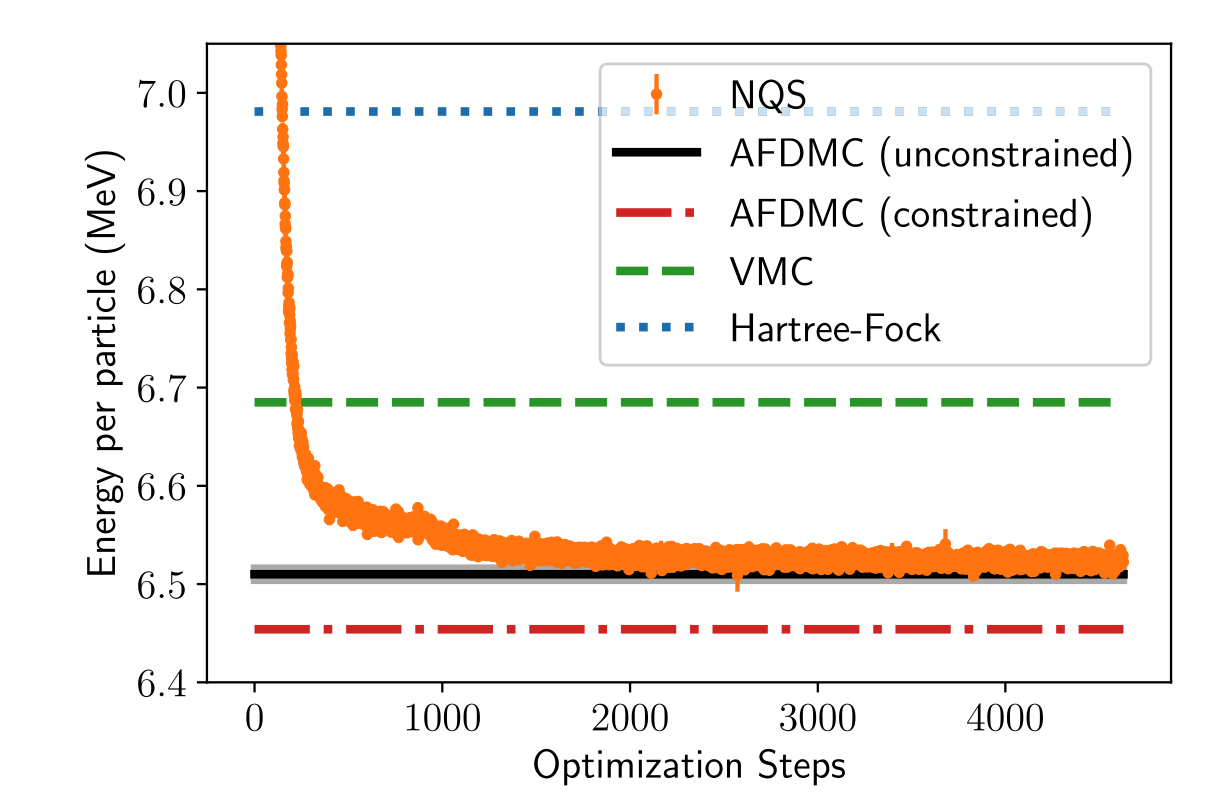
\includegraphics[width=0.9\linewidth]{figures/nmatter.png}}

\end{frame}


\begin{frame}[plain,fragile]
\frametitle{Self-emerging clustering Fore {\em et al.}, \url{https://www.nature.com/articles/s42005-025-02015-2}}
% inline figure
\centerline{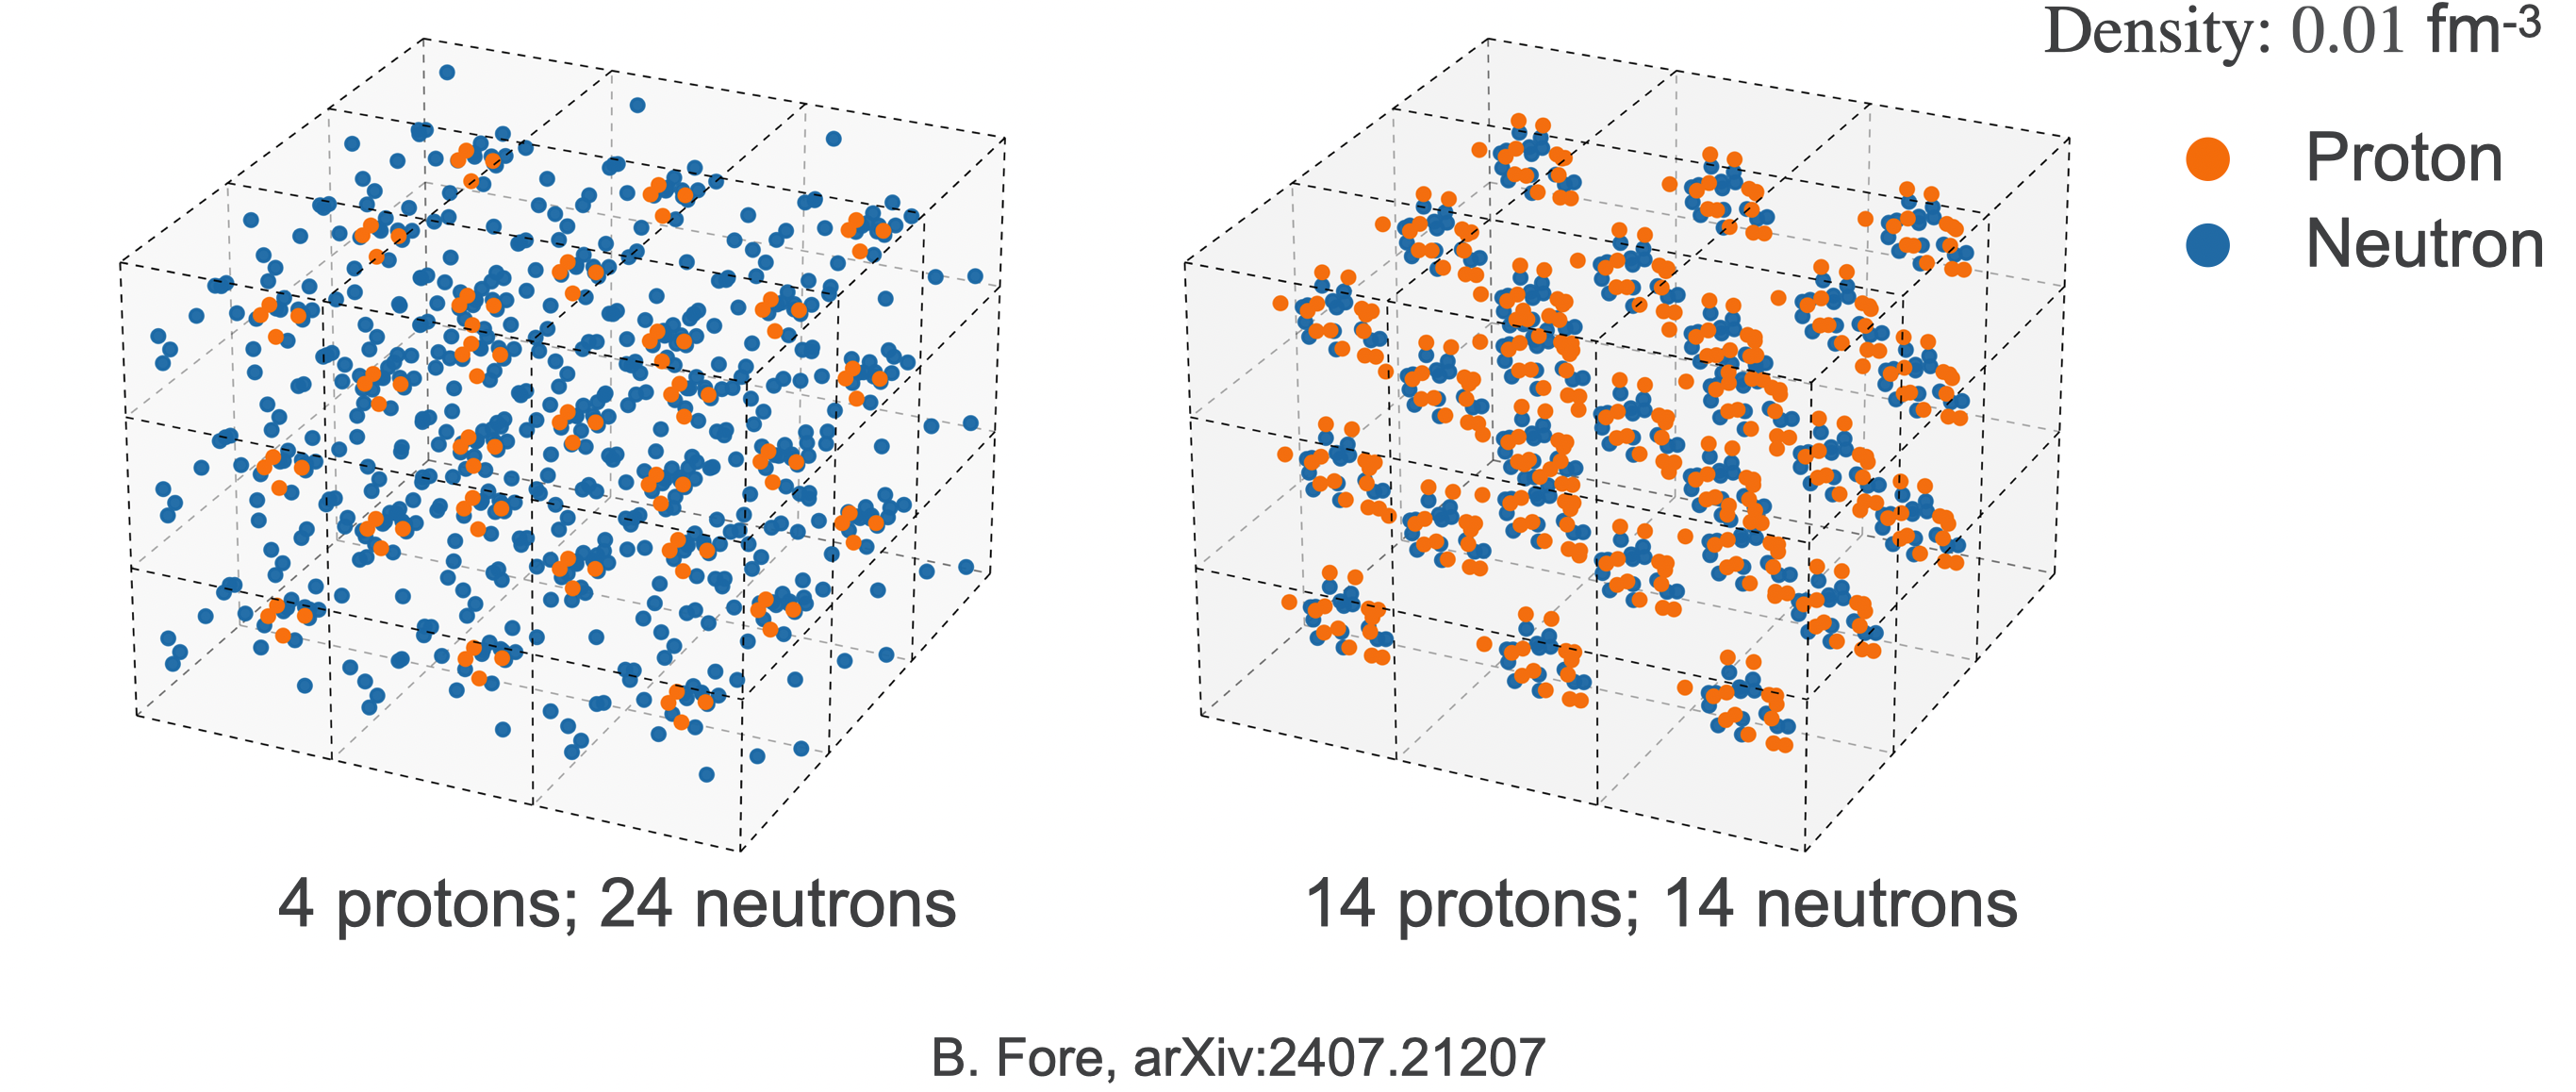
\includegraphics[width=1.0\linewidth]{figures/mbpfig7.png}}
\end{frame}


\begin{frame}[plain,fragile]
\frametitle{The electron gas in three dimensions with $N=14$ electrons (Wigner-Seitz radius $r_s=2$ a.u.), Kim {\em et al.},\url{https://journals.aps.org/prb/abstract/10.1103/PhysRevB.110.035108}}

\begin{block}{}
\centerline{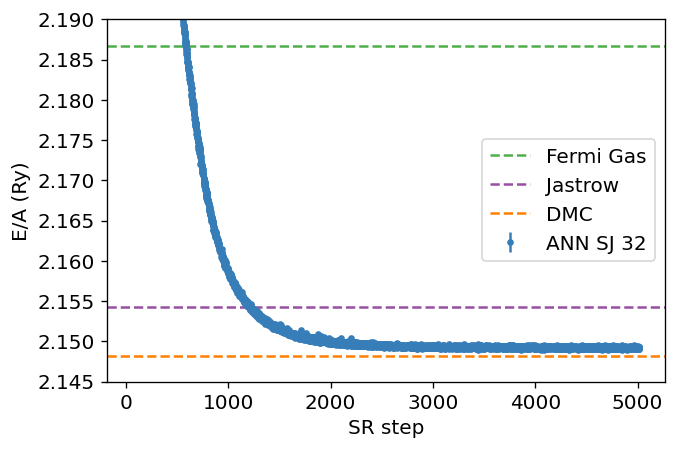
\includegraphics[width=0.8\linewidth]{figures/elgasnew.png}}

\end{block}
\end{frame}



\begin{frame}[plain,fragile]
\frametitle{And then quantum engineering and ML/AI}
\centerline{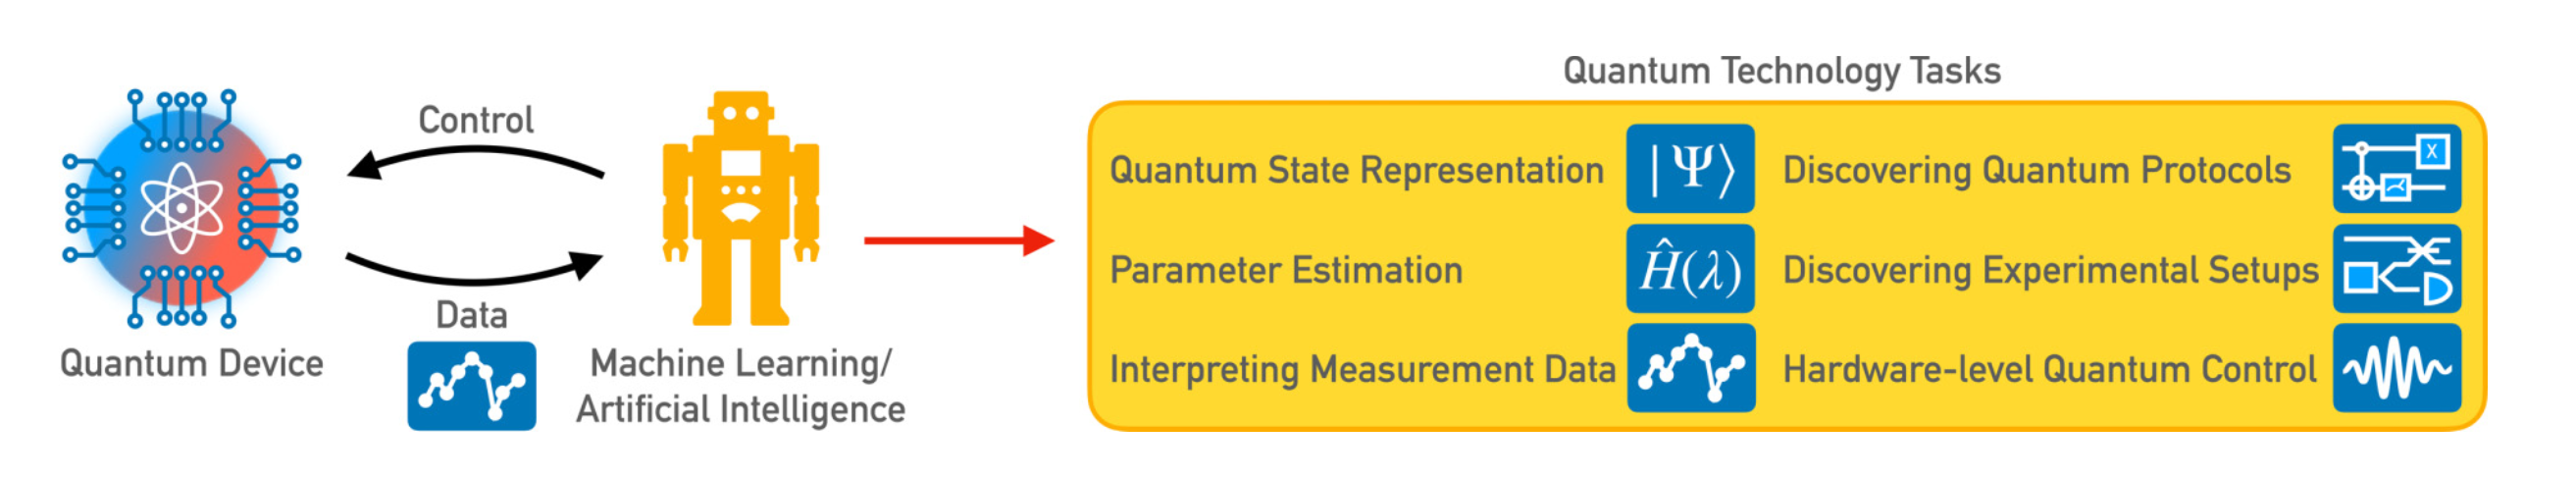
\includegraphics[width=1.05\linewidth]{figures/krenn1}}

\end{frame}


\begin{frame}{What is Quantum Entanglement?}
\textbf{Quantum Entanglement} is a quantum phenomenon where two or more particles become correlated in such a way that the state of one particle directly affects the state of the other, regardless of distance.

\vspace{10pt}
\textbf{Key Features:}
\begin{itemize}
    \item Non-local correlations
    \item No classical analog
    \item Violates Bell's inequalities
\end{itemize}

\textbf{Entangled State Example:}
\[
\ket{\Phi^+} = \frac{1}{\sqrt{2}} (\ket{00} + \ket{11})
\]

\end{frame}


\begin{frame}{1. Quantum Communication}
\textbf{Quantum Teleportation:}
\begin{itemize}
    \item Entanglement enables the transmission of quantum states using classical communication.
    \item No need to send the physical quantum particle.
\end{itemize}

\textbf{Advantage:}
\begin{itemize}
\item Instantaneous state transfer within quantum mechanics constraints.
\item Quantum networks rely on entanglement for secure communication.
  \end{itemize}
\end{frame}

\begin{frame}{2. Quantum Cryptography}
\textbf{Quantum Key Distribution:}
\begin{itemize}
    \item Entanglement ensures secure communication.
    \item Eavesdropping disturbs quantum states, revealing interception attempts.
\end{itemize}

\begin{itemize}
\item Any measurement by a third party collapses the wavefunction.  
\item Ensures security based on quantum mechanics, not computational hardness.
\end{itemize}
\textbf{Advantage:} Unconditional security guaranteed by the laws of physics.
\end{frame}

\begin{frame}{3. Quantum Computing}
\textbf{Speedup in Quantum Algorithms:}
\begin{itemize}
    \item Entanglement provides exponential state space.
    \item Quantum parallelism arises from entangled qubits.
\end{itemize}

\textbf{Grover's Algorithm:}
\[
\mathcal{O}(\sqrt{N}) \text{ vs. } \mathcal{O}(N)
\]

\textbf{Shor's Algorithm:}
\[
\text{Factoring in } \mathcal{O}((\log N)^3)
\]
\end{frame}

\begin{frame}[plain,fragile]
\frametitle{4. Quantum Metrology}

\textbf{Quantum Metrology:}
\begin{itemize}
    \item Uses entangled states for ultra-precise measurements.
    \item Overcomes the classical shot-noise limit.
\end{itemize}

\textbf{Heisenberg Limit:}
\[
\Delta \theta \ge \frac{1}{N},
\]

where \( N \) is the number of entangled particles.  

\begin{block}{Advantage:}
\begin{itemize}
\item Quantum entanglement improves sensitivity beyond classical limits.
\end{itemize}
\end{block}
\end{frame}

\begin{frame}{Challenges of Quantum Entanglement}
\textbf{Decoherence:}
\begin{itemize}
    \item Entangled states are fragile.
    \item Interaction with the environment collapses the wavefunction.
\end{itemize}

\textbf{Scalability:}
\begin{itemize}
    \item Difficult to entangle large numbers of qubits.
    \item Error correction requires complex protocols.
\end{itemize}

\textbf{Measurement Problem:}
\begin{itemize}
    \item Measurement destroys entanglement.
    \item Trade-off between information gain and entanglement preservation.
\end{itemize}
\end{frame}


\begin{frame}[plain,fragile]
\frametitle{Di Vincenzo criteria}

\begin{alertblock}{Quantum computing requirements }
\begin{enumerate}
\item A scalable physical system with well-characterized qubit

\item The ability to initialize the state of the qubits to a simple fiducial state

\item Long relevant Quantum coherence times longer than the gate operation time

\item A \textbf{universal} set of quantum gates

\item A qubit-specific measurement capability
\end{enumerate}

\noindent
\end{alertblock}
\end{frame}

\frame
    {
      \frametitle{Important properties, electrons on helium}
	
      \begin{footnotesize}
     \begin{columns}
       \column{5.0cm}
\begin{enumerate}
\item Long coherence times

\item Highly connect qubits

\item Many qubits in a small area

\item CMOS compatible

\item Fast gates
\end{enumerate}

\column{6cm}
      \begin{center}
	\rotatebox[origin=c]{-90}{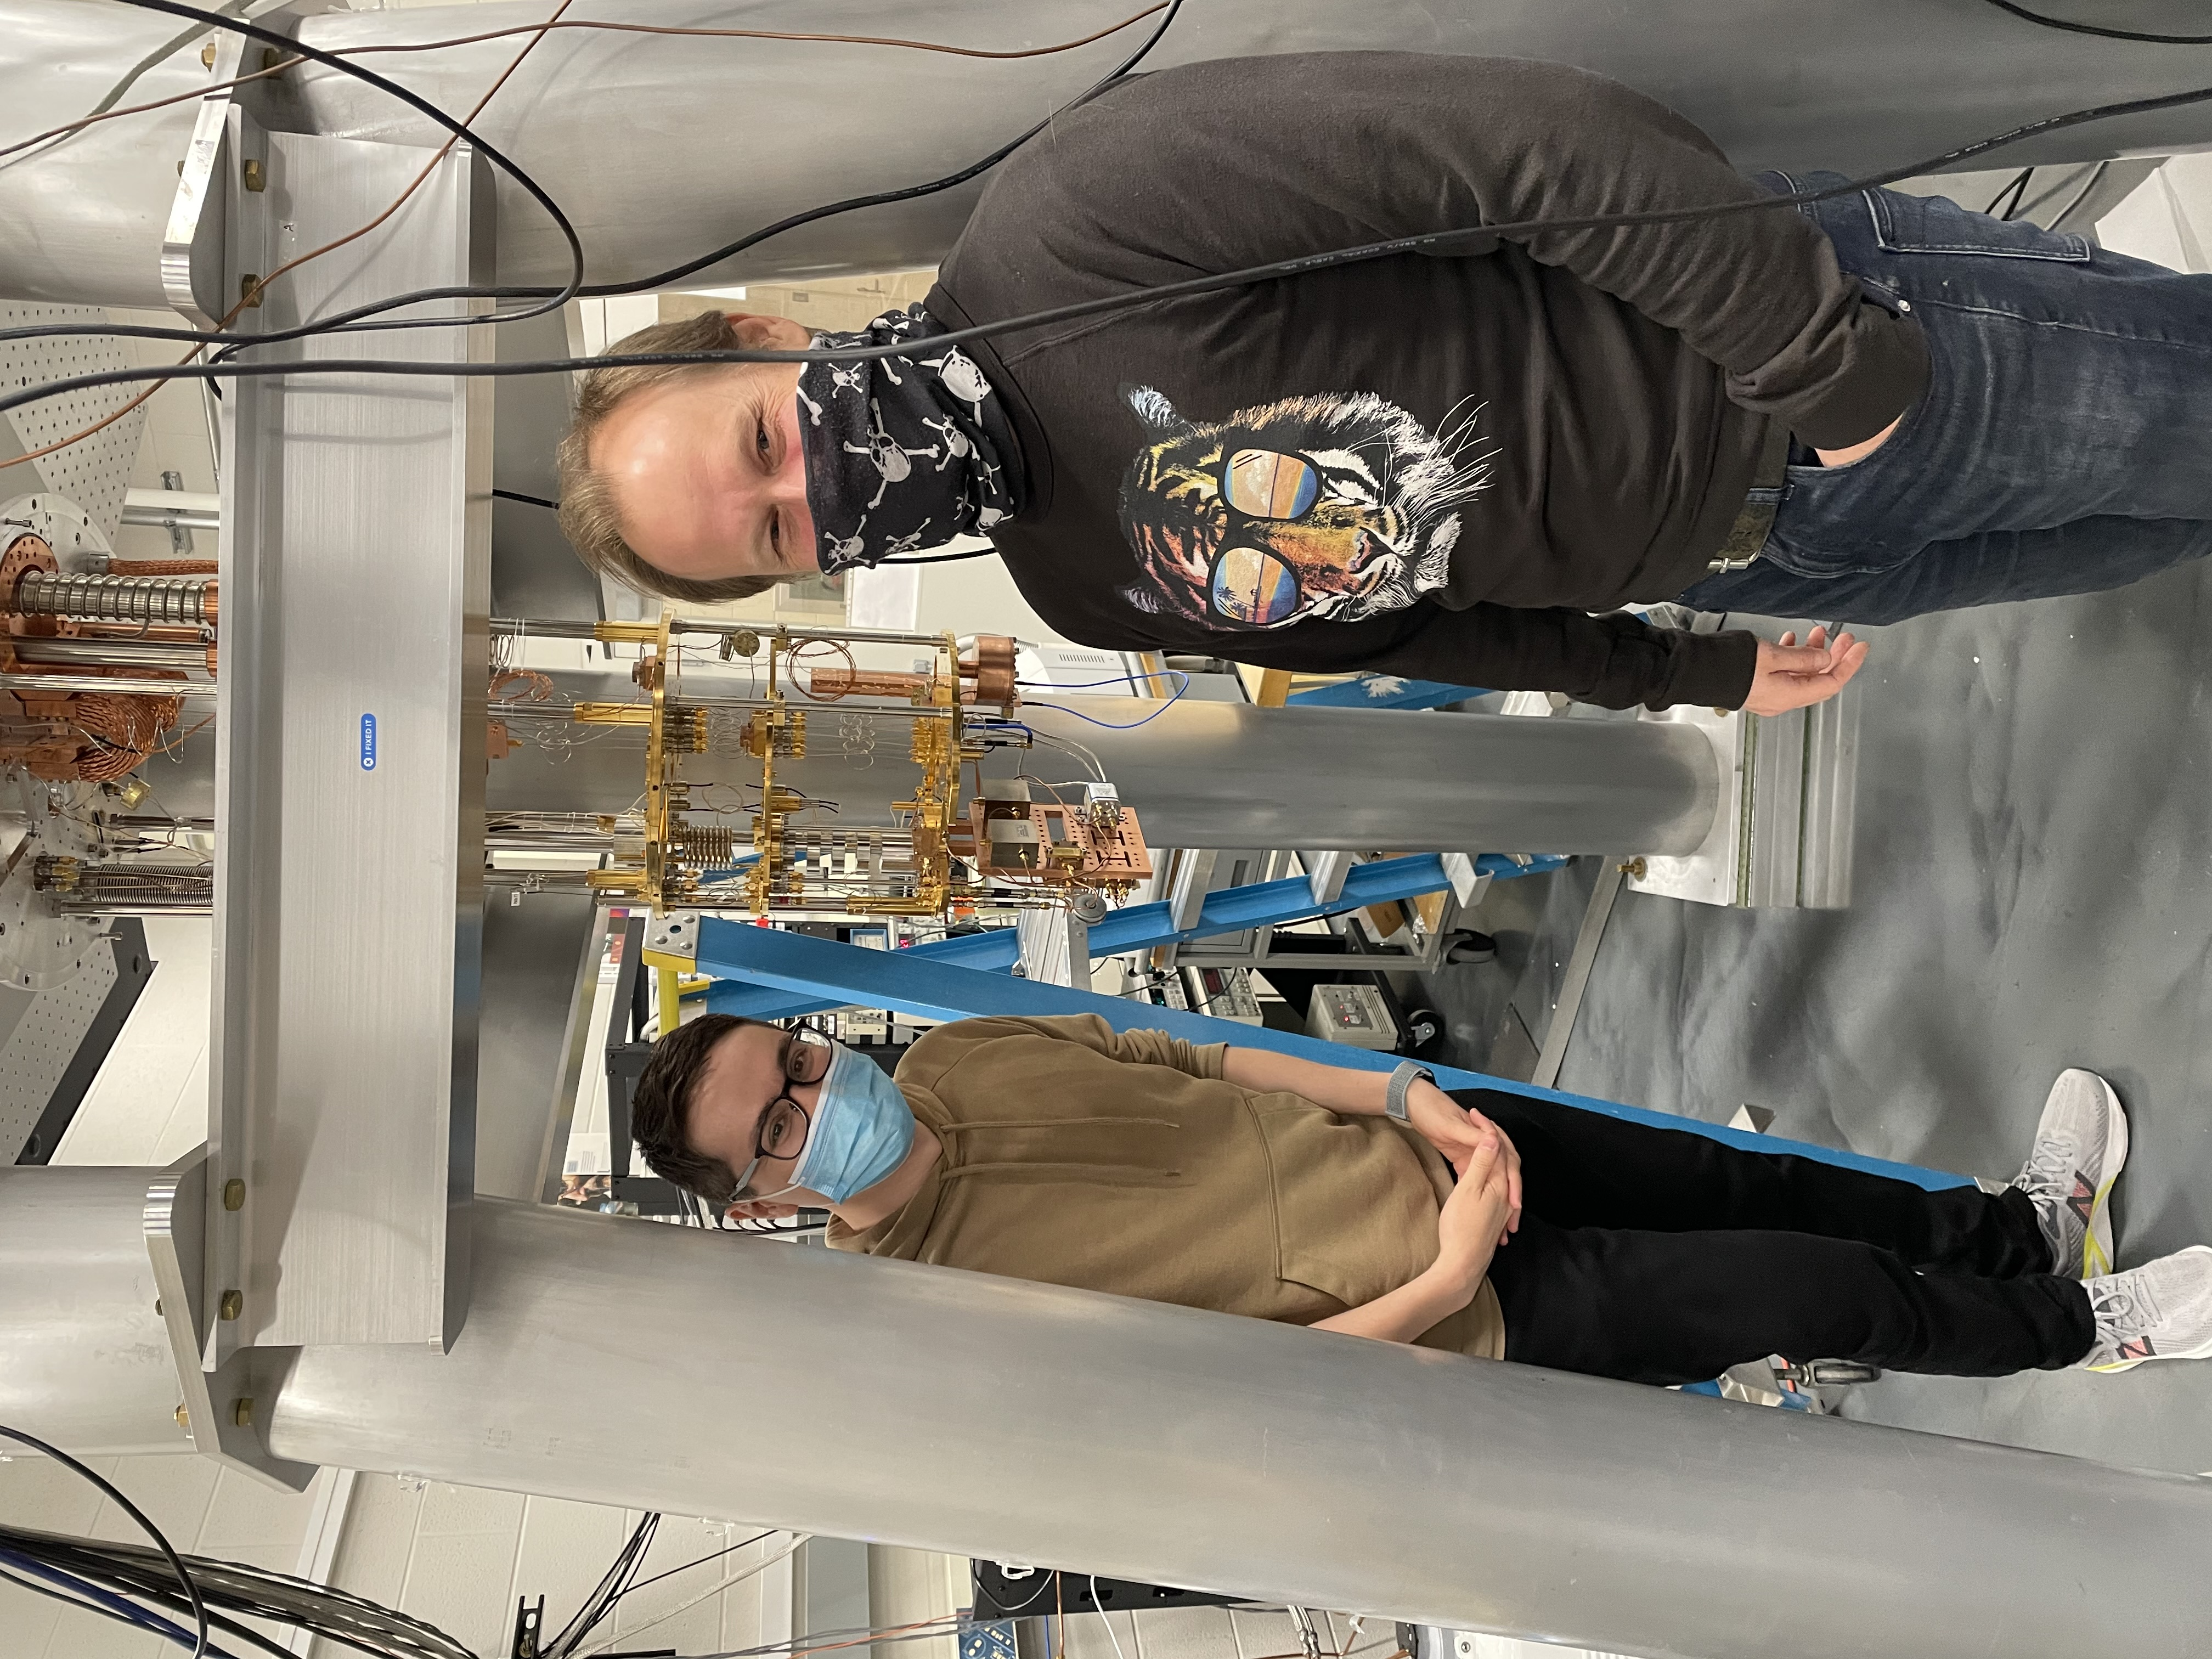
\includegraphics[width=1.3\textwidth]{qcfigures/lab.jpeg}}
      \end{center}
\end{columns}
      \end{footnotesize}
    }




\frame
    {
      \frametitle{Single electrons can make great qubits}
	
      \begin{footnotesize}
     \begin{columns}
       \column{5.0cm}

       At the heart is the trapping and control
       of individual electrons floating above pools of superfluid
       helium. These electrons form the qubits of our quantum
       computer, and the purity of the superfluid helium protects the
       intrinsic quantum properties of each electron. The  ultimate
       goal is to build a large-scale quantum computer based on
       quantum magnetic (spin) state of these trapped electrons.
\column{5cm}
      \begin{center}
	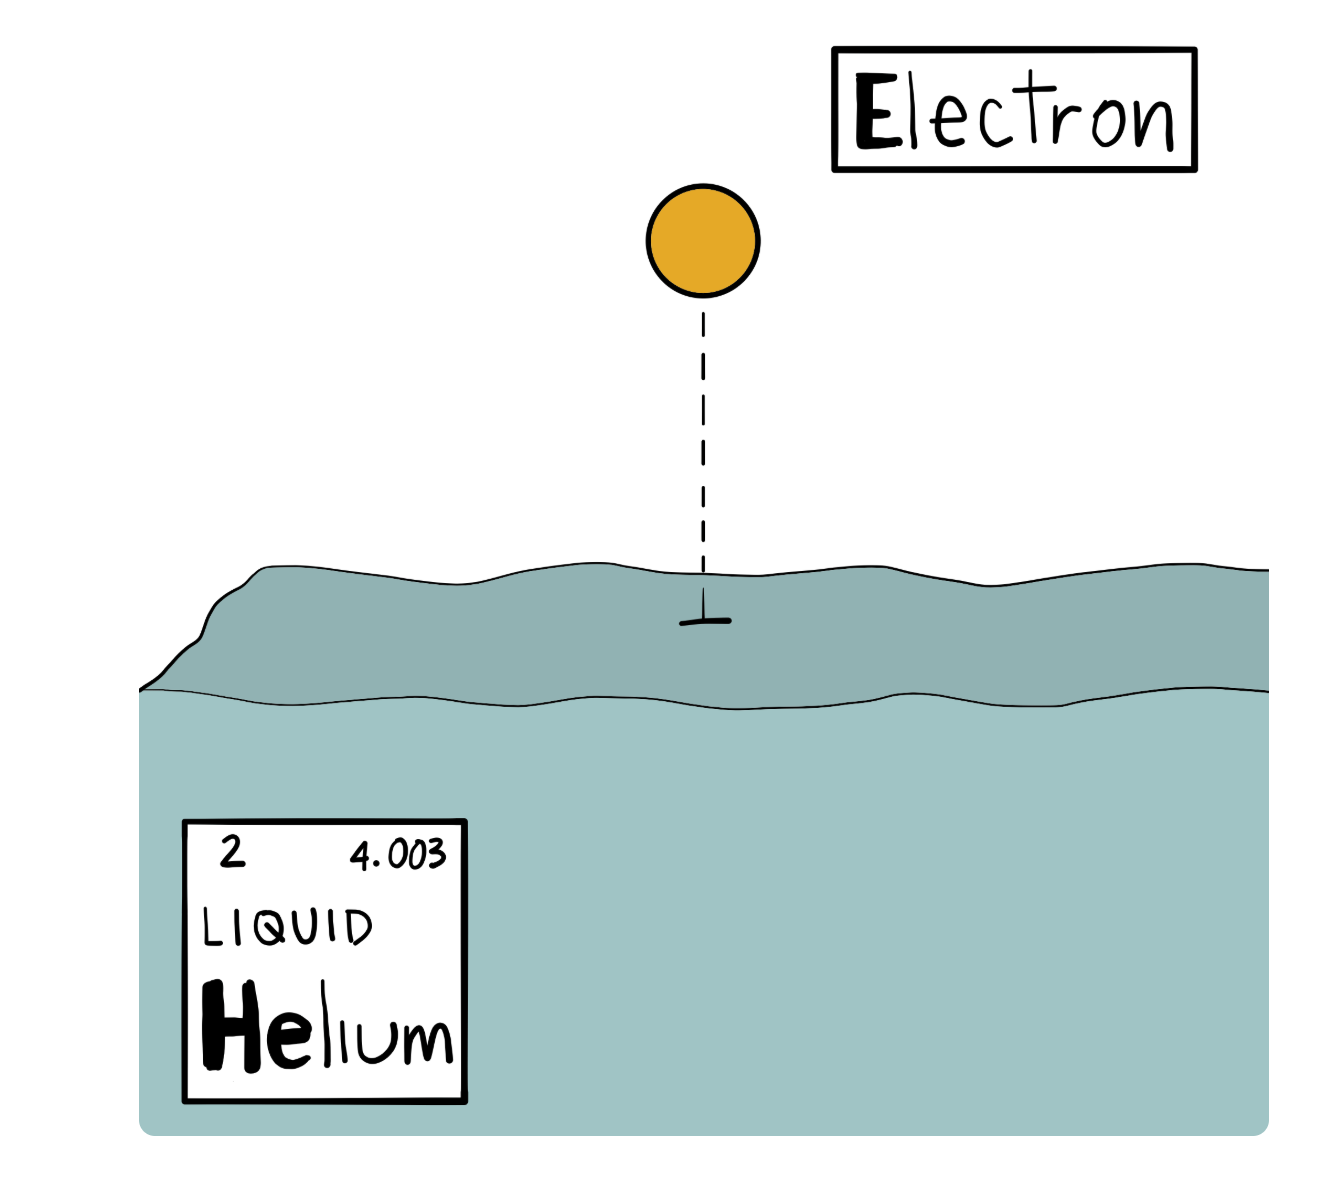
\includegraphics[width=1.2\textwidth]{qcfigures/nordicquantumfig1.png}
      \end{center}
\end{columns}
      \end{footnotesize}
    }


\frame
    {
      \frametitle{Trapping electrons in microchannels}
	
      \begin{footnotesize}
     \begin{columns}
       \column{5.0cm}
Microchannels fabricated into silicon wafers are filled with superfluid helium and energized electrodes. Together with the natural electron trapping properties of superfluid helium, these allow for the precision trapping of individual or multiple electrons. The microchannels are only a few micrometers in size, or about five times smaller than the diameter of a human hair.
\column{5cm}
      \begin{center}
	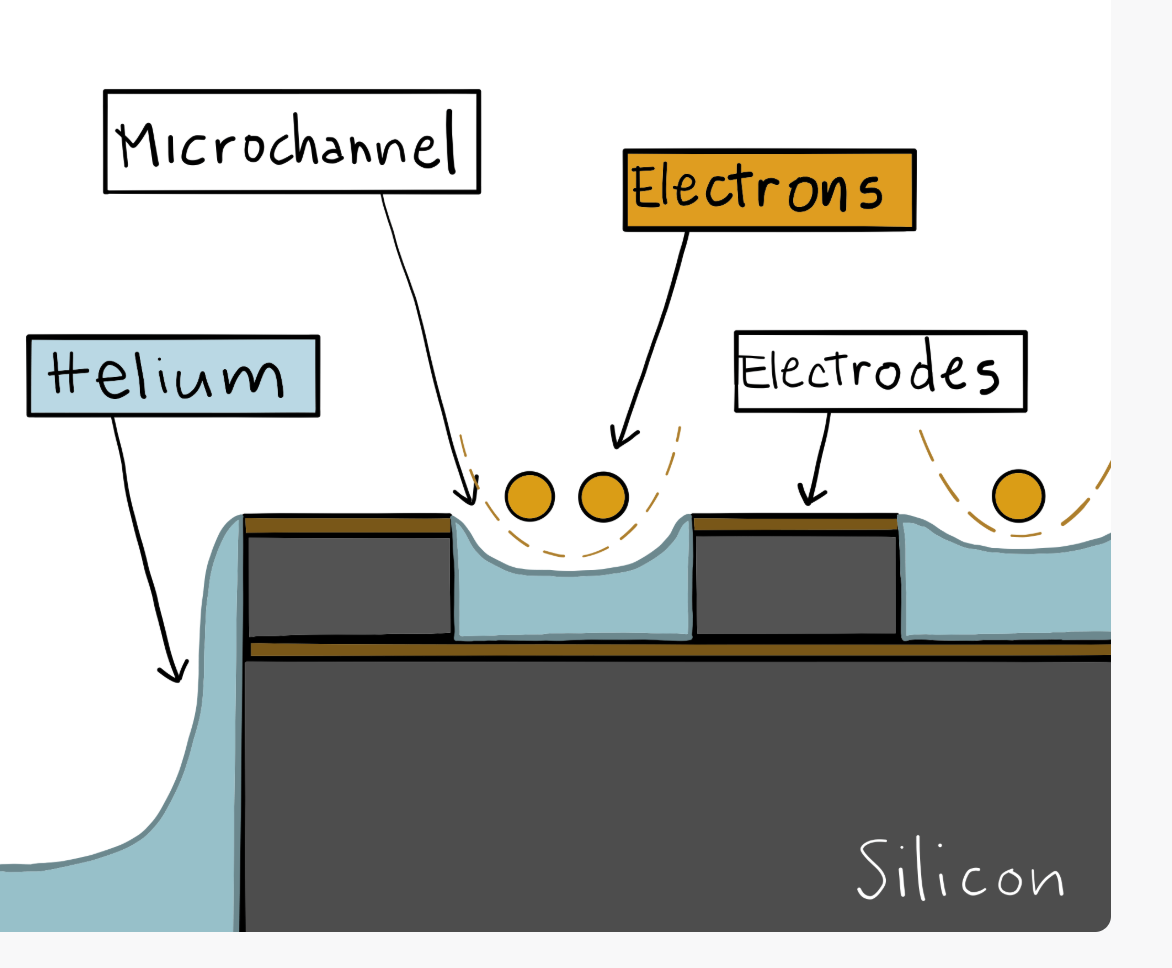
\includegraphics[width=1.2\textwidth]{qcfigures/nordicquantumfig2.png}
      \end{center}
\end{columns}
      \end{footnotesize}
    }

\frame
    {
      \frametitle{Control and readout}
	
      \begin{footnotesize}
     \begin{columns}
       \column{5.0cm}

       Microchannel regions can store thousands of electrons, from which one can be plucked and transported to the single electron control and readout area. In this region, microwave signals will interact with the electron to perform quantum logic gate operations, which will be readout via extremely fast electronics.


\column{5cm}
      \begin{center}
	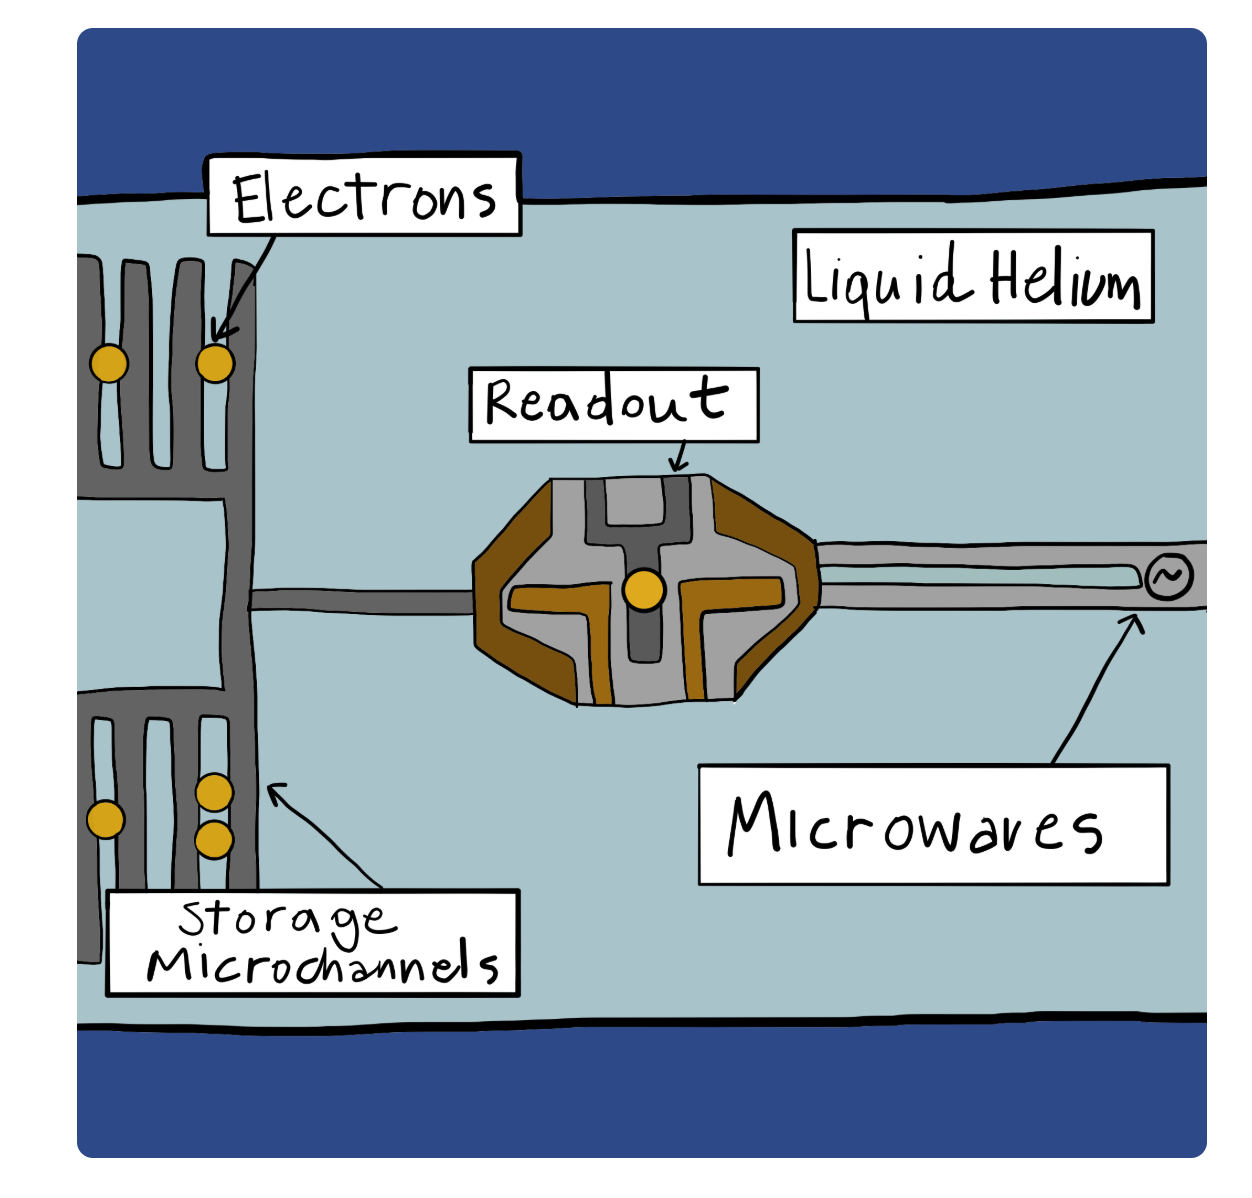
\includegraphics[width=1.2\textwidth]{qcfigures/nordicquantumfig3.png}
      \end{center}
\end{columns}
      \end{footnotesize}
    }


\frame
    {
      \frametitle{Operations for quantum computing}
	
      \begin{footnotesize}
     \begin{columns}
       \column{5.0cm}
Quantum information can be encoded in a number of ways using single electrons. Currently, we are working with the side-to-side(lateral) quantum motion of the electron in the engineered trap. This motion can either be in its lowest energy state, the ground state, or in a number of higher-energy excited states. This electron motion also provides the readout capabilities for the ultimate goal of building a large-scale quantum computer based on the electron's magnetic moment (spin).       
\column{5cm}
      \begin{center}
	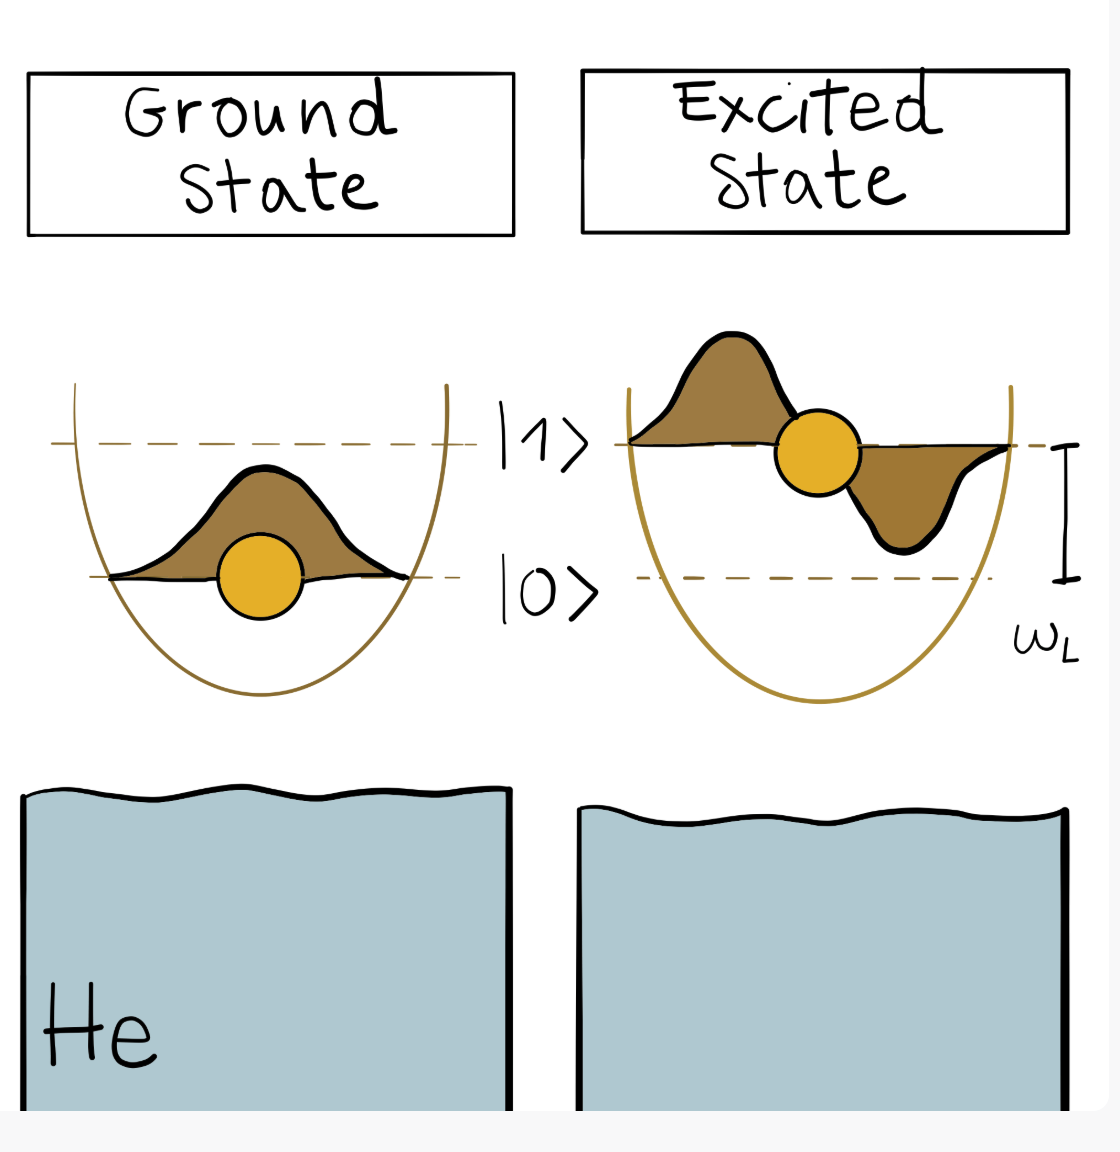
\includegraphics[width=1.2\textwidth]{qcfigures/nordicquantumfig4.png}
      \end{center}
\end{columns}
      \end{footnotesize}
    }
    
\section{Experiment and theory}




\begin{frame}[plain,fragile]
\frametitle{Qubit platforms}

\vspace{6mm}

% inline figure
\centerline{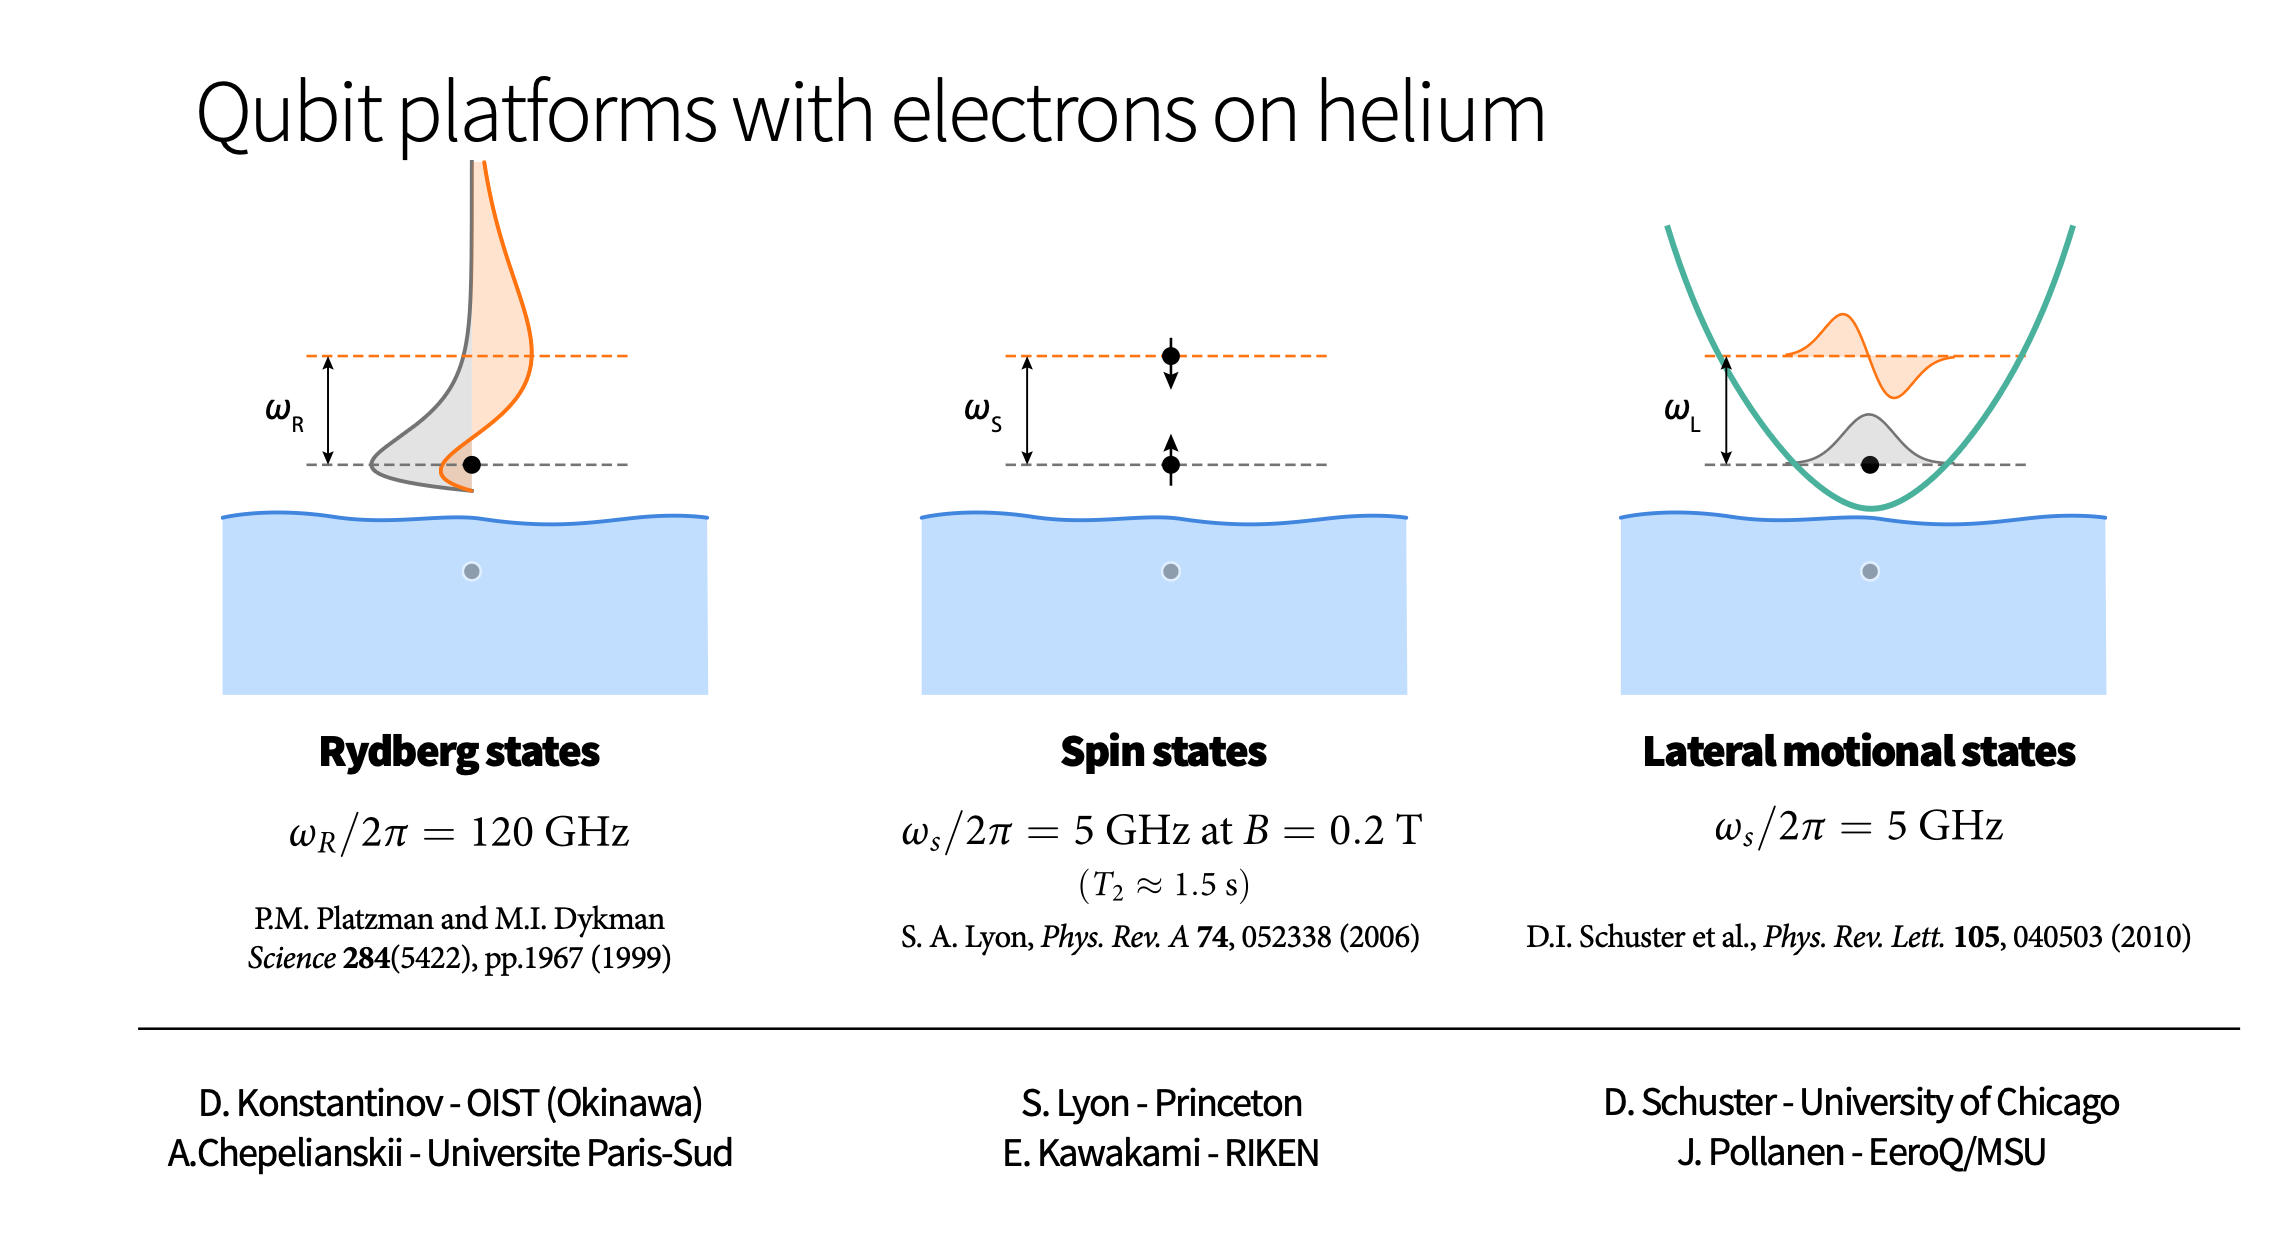
\includegraphics[width=1.2\linewidth]{qcfigures/Elhelium2.png}}

\vspace{6mm}
\end{frame}

\frame
    {
      \frametitle{Final experimental setup}
	
      \begin{footnotesize}
     \begin{columns}
       \column{5.0cm}
\begin{enumerate}
\item (a) Microdevice where two electrons are trapped in a double-well potential created by electrodes 1-7. The read-out is provided by two superconducting resonators dispersively coupled to  electron's in-plane motional states.

\item (b) Coupling constants from each individual electrode beneath the helium layer.

\item (c+d) The electron's energy in a  double-well electrostatic potential. 
\end{enumerate}

\column{6cm}
      \begin{center}
	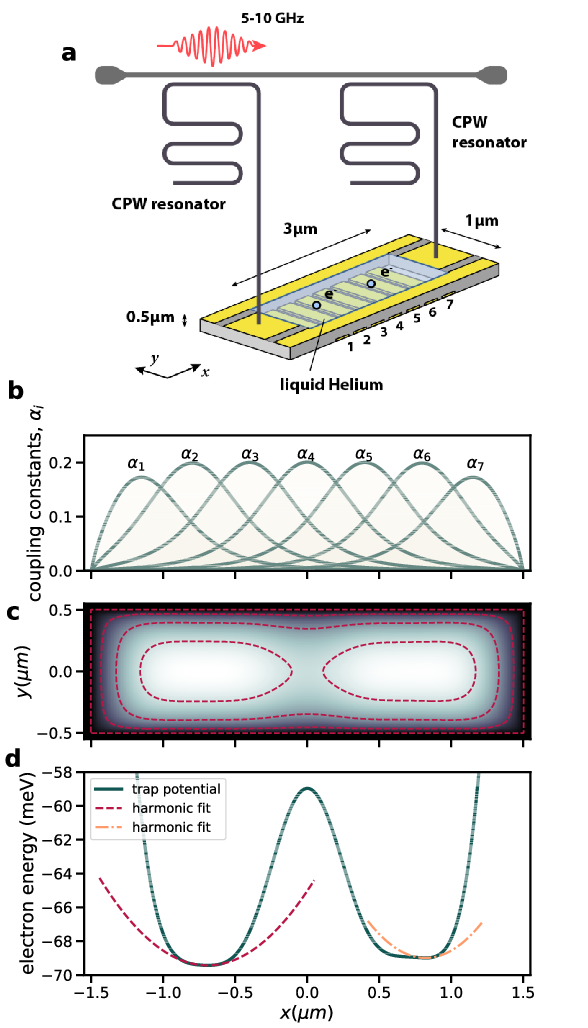
\includegraphics[width=0.65\textwidth]{qcfigures/figure1.png}
      \end{center}
\end{columns}
      \end{footnotesize}
    }




\begin{frame}[plain,fragile]
\frametitle{Two-qubit gates and time evolution, SWAP gate}
% inline figure
\centerline{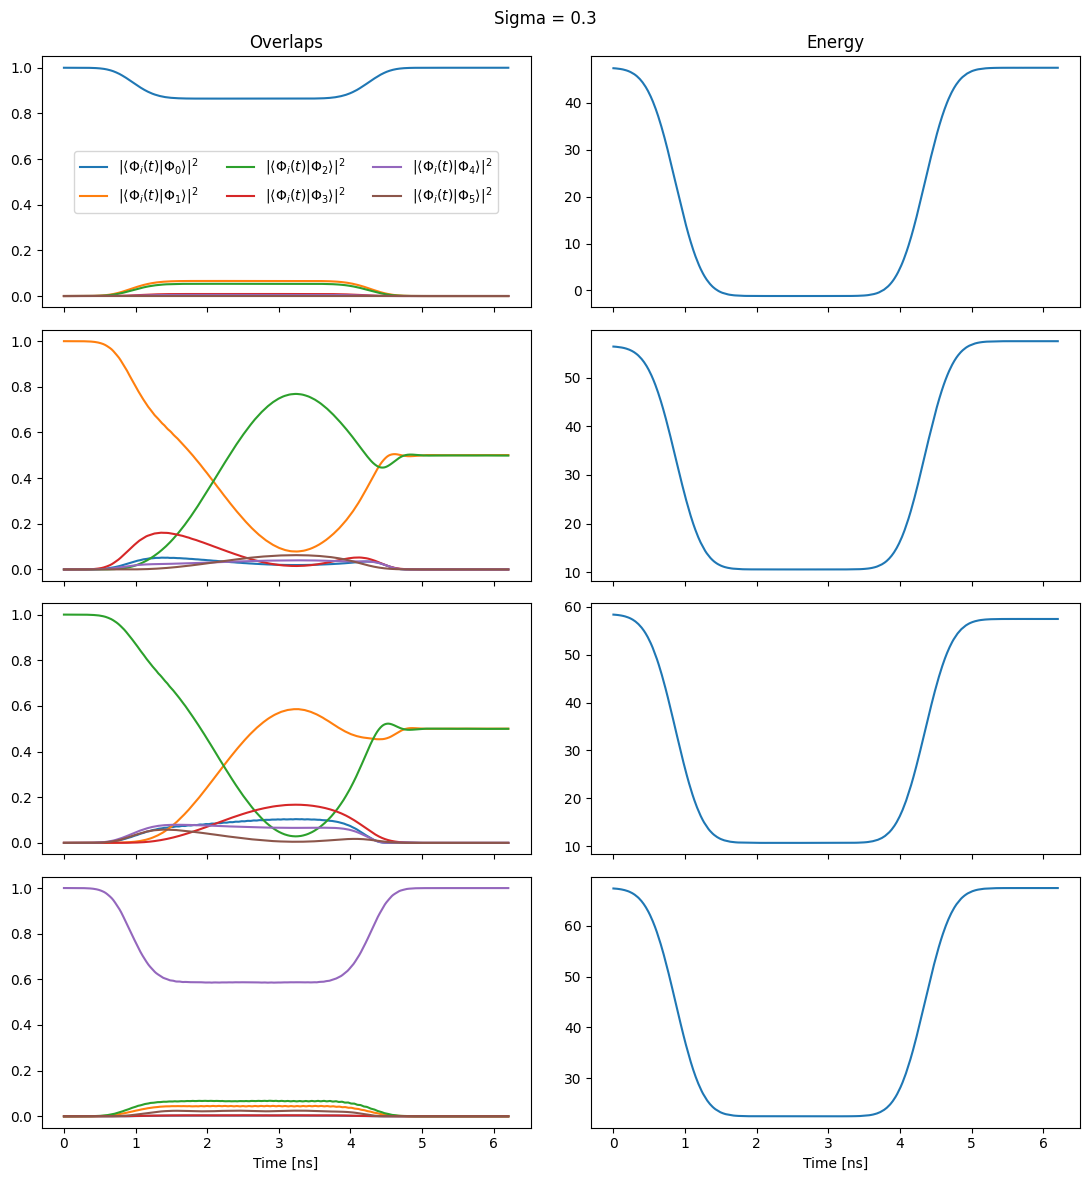
\includegraphics[width=0.65\linewidth]{qcfigures/timeevolution.png}}
\end{frame}














\begin{frame}[plain,fragile]
\frametitle{Observations (or conclusions if you prefer)}


\begin{block}{}
\begin{itemize}
\item How do we develop insights, competences, knowledge in AI and quantum technologies  that can advance a given field?
\begin{itemize}

  \item For example: Can we use ML to find out which correlations are relevant and thereby diminish the dimensionality problem in complex interacting  many-particle systems?

  \item Can we use AI/ML in detector analysis, accelerator design, analysis of experimental data and more?

  \item Can we use AL/ML to carry out reliable extrapolations by using current experimental knowledge and current theoretical models?
\item How do we study entanglement in various quantum platforms? Can we use AI/ML for better design?

\end{itemize}

\noindent
\item The community needs to invest in relevant educational efforts and training of scientists with knowledge in AI/ML and quantum technologies

\item Most likely tons of things I have forgotten
\end{itemize}

\noindent
\end{block}
\end{frame}

\begin{frame}{More conclusions or perspectives: Selected applications of Quantum Machine Learning}
\textbf{1. Quantum mechanical many-particle systems:}
\begin{itemize}
    \item Simulate  structures in nuclei, atoms, moleculs etc with QML.
\end{itemize}

\textbf{2. Finance:}
\begin{itemize}
    \item Quantum optimization for portfolio management.
\end{itemize}

\textbf{3. Image Recognition:}
\begin{itemize}
    \item Quantum-enhanced convolutional neural networks.
\end{itemize}
\end{frame}


\begin{frame}[plain,fragile]
\frametitle{Thank you for the attention and results from references in slides)}
\begin{enumerate}

\item Bryce Fore, Jane Kim, Morten Hjorth-Jensen, Alessandro Lovato, \textbf{Investigating the crust of neutron stars with neural-network quantum states}, Communications Physics \textbf{8}, 108  (2025) and \href{{https://www.nature.com/articles/s42005-025-02015-2}}{\nolinkurl{https://www.nature.com/articles/s42005-025-02015-2}}

\item Patrick Cook, Danny Jammooa, Morten Hjorth-Jensen, Daniel D. Lee, Dean Lee, \textbf{Parametric Matrix Models}, Nature Communications  under review and \href{{https://arxiv.org/abs/2401.11694}}{\nolinkurl{https://arxiv.org/abs/2401.11694}}

\item Niyaz R. Beysengulov, Johannes Pollanen, Øyvind S. Schøyen, Stian D. Bilek, Jonas B. Flaten, Oskar Leinonen, Håkon Emil Kristiansen, Zachary J. Stewart, Jared D. Weidman, Angela K. Wilson, Morten Hjorth-Jensen, Coulomb interaction-driven entanglement of electrons on helium, PRX Quantum 5, 030324 (2024) and \href{{https://journals.aps.org/prxquantum/abstract/10.1103/PRXQuantum.5.030324}}{\nolinkurl{https://journals.aps.org/prxquantum/abstract/10.1103/PRXQuantum.5.030324}}

\end{enumerate}
\end{frame}



\begin{frame}[plain,fragile]
\frametitle{Additional references)}
\begin{enumerate}

\item Jane Kim, Gabriel Pescia, Bryce Fore, Jannes Nys, Giuseppe Carleo, Stefano Gandolfi, Morten Hjorth-Jensen, Alessandro Lovato, \textbf{Neural-network quantum states for ultra-cold Fermi gases}, Communications Physics \textbf{7}, 148 (2024) and \href{{https://www.nature.com/articles/s42005-024-01613-w}}{\nolinkurl{https://www.nature.com/articles/s42005-024-01613-w}}

\item Bryce Fore, Jane M. Kim, Giuseppe Carleo, Morten Hjorth-Jensen, Alessandro Lovato, and Maria Piarulli, \textbf{Dilute neutron star matter from neural-network quantum states}, \href{{https://journals.aps.org/prresearch/abstract/10.1103/PhysRevResearch.5.033062}}{Physical Review  Research 5, 033062 (2023)}

\item Robert Solli, Daniel Bazin, Michelle P. Kuchera, Ryan R. Strauss, Morten Hjorth-Jensen, \emph{Unsupervised Learning for Identifying Events in Active Target Experiments}, \href{{https://www.sciencedirect.com/science/article/abs/pii/S0168900221004460}}{Nuclear Instruments and Methods in Physics Research Section A \textbf{1010}, 165461, (2020)}

\end{enumerate}
\end{frame}


\appendix{Additional material}






\begin{frame}{1. Quantum Support Vector Machines (QSVM)}
\textbf{Quantum Kernel Estimation:}
\begin{itemize}
    \item Maps classical data to a quantum Hilbert space.
    \item Quantum kernel measures similarity in high-dimensional space.
\end{itemize}

\pause
\textbf{Quantum Kernel:}
\[
K(x, x') = |\braket{\psi(x) | \psi(x')}|^2
\]

\textbf{Advantage:}
- Potentially exponential speedup over classical SVMs.
\end{frame}

\begin{frame}{2. Quantum Neural Networks (QNNs)}
\textbf{Quantum Neural Networks} replace classical neurons with parameterized quantum circuits.

\textbf{Key Concepts:}
\begin{itemize}
    \item Quantum Gates as Activation Functions.
    \item Variational Quantum Circuits (VQCs) for optimization.
\end{itemize}

\pause
\textbf{Parameterized Quantum Circuit:}
\[
U(\theta) = \prod_i R_y(\theta_i) \cdot CNOT \cdot R_x(\theta_i)
\]

\textbf{Advantage:}
- Quantum gradients enable exploration of non-convex landscapes.
\end{frame}

\begin{frame}{3. Quantum Boltzmann Machines (QBMs)}
\textbf{Quantum Boltzmann Machines} leverage quantum mechanics to sample from a probability distribution.

\begin{itemize}
    \item Quantum tunneling aids in escaping local minima.
    \item Quantum annealing for optimization problems.
\end{itemize}

\pause
\textbf{Quantum Hamiltonian:}
\[
H = -\sum_i b_i \sigma_i^z - \sum_{ij} w_{ij} \sigma_i^z \sigma_j^z
\]

\textbf{Advantage:}
- Efficient sampling in complex probability distributions.
\end{frame}


\section{Future Perspectives}
\begin{frame}{Future Perspectives in QML}
\textbf{1. Fault-Tolerant Quantum Computing:}
\begin{itemize}
    \item Overcoming noise for stable quantum circuits.
\end{itemize}

\textbf{2. Hybrid Quantum-Classical Models:}
\begin{itemize}
    \item Combining quantum circuits with classical neural networks.
\end{itemize}

\textbf{3. Quantum Internet:}
\begin{itemize}
    \item Distributed quantum machine learning over quantum networks.
\end{itemize}
\end{frame}
















\begin{frame}[plain,fragile]
\frametitle{Universal approximation theorem}

The universal approximation theorem plays a central role in deep
learning.  \href{{https://link.springer.com/article/10.1007/BF02551274}}{Cybenko (1989)} showed
the following:

\begin{block}{}
Let $\sigma$ be any continuous sigmoidal function such that
\[
\sigma(z) = \left\{\begin{array}{cc} 1 & z\rightarrow \infty\\ 0 & z \rightarrow -\infty \end{array}\right.
\]
Given a continuous and deterministic function $F(\bm{x})$ on the unit
cube in $d$-dimensions $F\in [0,1]^d$, $x\in [0,1]^d$ and a parameter
$\epsilon >0$, there is a one-layer (hidden) neural network
$f(\bm{x};\bm{\Theta})$ with $\bm{\Theta}=(\bm{W},\bm{b})$ and $\bm{W}\in
\mathbb{R}^{m\times n}$ and $\bm{b}\in \mathbb{R}^{n}$, for which
\[
\vert F(\bm{x})-f(\bm{x};\bm{\Theta})\vert < \epsilon \hspace{0.1cm} \forall \bm{x}\in[0,1]^d.
\]

\end{block}
\end{frame}

\begin{frame}[plain,fragile]
\frametitle{The approximation theorem in words}

\textbf{Any continuous function $y=F(\bm{x})$ supported on the unit cube in
$d$-dimensions can be approximated by a one-layer sigmoidal network to
arbitrary accuracy.}

\href{{https://www.sciencedirect.com/science/article/abs/pii/089360809190009T}}{Hornik (1991)} extended the theorem by letting any non-constant, bounded activation function to be included using that the expectation value
\[
\mathbb{E}[\vert F(\bm{x})\vert^2] =\int_{\bm{x}\in D} \vert F(\bm{x})\vert^2p(\bm{x})d\bm{x} < \infty.
\]
Then we have
\[
\mathbb{E}[\vert F(\bm{x})-f(\bm{x};\bm{\Theta})\vert^2] =\int_{\bm{x}\in D} \vert F(\bm{x})-f(\bm{x};\bm{\Theta})\vert^2p(\bm{x})d\bm{x} < \epsilon.
\]
\end{frame}

\begin{frame}[plain,fragile]
\frametitle{More on the general approximation theorem}

None of the proofs give any insight into the relation between the
number of of hidden layers and nodes and the approximation error
$\epsilon$, nor the magnitudes of $\bm{W}$ and $\bm{b}$.

Neural networks (NNs) have what we may call a kind of universality no matter what function we want to compute.

\begin{block}{}
It does not mean that an NN can be used to exactly compute any function. Rather, we get an approximation that is as good as we want. 
\end{block}
\end{frame}

\begin{frame}[plain,fragile]
\frametitle{Class of functions we can approximate}

\begin{block}{}
The class of functions that can be approximated are the continuous ones.
If the function $F(\bm{x})$ is discontinuous, it won't in general be possible to approximate it. However, an NN may still give an approximation even if we fail in some points.
\end{block}
\end{frame}

\end{document}

%-----------------------------------------------------------
\section{Future Perspectives}
\begin{frame}{Future Perspectives}
\textbf{Quantum Internet:}
\begin{itemize}
    \item Entanglement as a resource for global quantum networks.
\end{itemize}

\textbf{Fault-Tolerant Quantum Computing:}
\begin{itemize}
    \item Quantum error correction leveraging entanglement.
\end{itemize}

\textbf{Advanced Quantum Sensors:}
\begin{itemize}
    \item Improved sensitivity for medical and scientific applications.
\end{itemize}

\pause
\textbf{Conclusion:}
- Quantum entanglement is a fundamental resource.  
- It enables quantum supremacy in communication, computation, and sensing.
\end{frame}







Based on a detailed review of the article **“Strong coupling of a microwave photon to an electron on helium” (arXiv:2509.14506v1)** and its supplementary materials, the **technological components potentially subject to export control regulations** (such as under the U.S. **Export Administration Regulations (EAR)**, EU **Dual-Use Regulation (EU) 2021/821**, or Norwegian equivalents) are the following:

---

### **1. Superconducting Quantum Microwave Devices**

* **High-impedance superconducting resonator** (fabricated from **titanium nitride (TiN)** and **niobium (Nb)** nanowires).

  * These are **superconducting microwave resonators** designed for strong coupling to quantum systems.
  * Controlled under export lists when used in **quantum computing**, **high-frequency detection**, or **quantum-limited measurement** systems (ECCN 3A991/3A231 or EU Category 3A001.b.10).

---

### **2. Quantum Control and Measurement Electronics**

* **Cryogenic microwave circuitry** including high-electron mobility transistor (**HEMT**) amplifiers, **bias tees**, and **microwave filters** capable of operation below 10 mK.

  * Such systems are part of **quantum-limited cryogenic readout** chains for qubit measurement and can fall under export controls as **quantum-limited amplifiers** or **quantum sensing components**.

---

### **3. Quantum Dot and Trapping System**

* **Electrostatic trapping and control of single electrons on superfluid helium**, integrated into a **microfabricated silicon-based microfluidic platform**.

  * These devices implement **quantum confinement** and **precision charge control**, key enabling technologies for **quantum information processing**.
  * Falls under **dual-use classification for quantum information systems** (ECCN 3E001 or EU 3E001, technology for the development of quantum computing devices).

---

### **4. Fabrication and Design Technology**

* **Electron-beam lithography and reactive-ion etching (RIE) methods** for patterning TiN/Nb superconducting circuits with sub-micrometer resolution.

  * Such fabrication know-how and associated CAD/FEM simulation tools (e.g., finite element models of qubit–resonator coupling) may be classified under **3E002** (“technology for development or production of superconducting electronics”).

---

### **5. Cryogenic and Quantum Experimental Systems**

* **Dilution refrigerator systems (Bluefors LD400)** operating below 10 mK with integrated **quantum microwave lines**, filters, and bias systems.

  * While the refrigerator itself is not normally export-restricted, **integration into quantum computing or quantum sensing architectures** may invoke **dual-use provisions**.

---

### **Summary of Export-Relevant Elements**

| Category                         | Component                                                            | Potential Control Reference |
| -------------------------------- | -------------------------------------------------------------------- | --------------------------- |
| Superconducting quantum circuits | TiN/Nb high-impedance resonators                                     | 3A991.b.2 / 3A231           |
| Quantum control electronics      | Cryogenic HEMT amplifiers, bias tees, low-noise microwave components | 3A001.b.10                  |
| Quantum devices                  | Electron-on-helium quantum dots and coupling schemes                 | 3E001 / 3E002               |
| Fabrication technology           | E-beam lithography, RIE, FEM-based quantum design                    | 3E002                       |
| Cryogenic systems                | Dilution refrigerator integration with quantum hardware              | 3B001 or “use” under 3E001  |

---

### **Non-Controlled Scientific Aspects**

The *scientific data, published results,* and *basic research* aspects of this work—such as theoretical models, FEM simulations, and open-source software repositories (e.g., **ZeroHeliumKit**, **Quantum Electron**)—are **not subject to export control** under the research exemption for publicly available fundamental research.

---

Would you like me to prepare a **one-page summary table** (formatted for a grant or compliance document) that clearly lists these components, control categories, and justifications?



Here’s a **one-page summary table** outlining the **technological components in the article** *“Strong coupling of a microwave photon to an electron on helium” (arXiv:2509.14506v1)* that may be influenced by **export control regulations** (e.g., EU Dual-Use Regulation 2021/821, EAR, or Norwegian equivalents).

---

## **Export Control Summary – Technological Components in “Strong Coupling of a Microwave Photon to an Electron on Helium”**

| **Category**                             | **Component / Technology**                                                          | **Description and Use**                                                                                                     | **Potential Export Control Relevance**                                                                                          | **Indicative Control Reference**        |
| ---------------------------------------- | ----------------------------------------------------------------------------------- | --------------------------------------------------------------------------------------------------------------------------- | ------------------------------------------------------------------------------------------------------------------------------- | --------------------------------------- |
| **1. Superconducting Quantum Circuits**  | High-impedance **TiN/Nb superconducting resonators**                                | Nanofabricated microwave resonators enabling strong coupling between single electrons and photons at GHz frequencies.       | Considered **quantum-limited superconducting electronics**; restricted when used for quantum computing or sensing applications. | EU 3A001.b.10 / EAR 3A991.b.2 or 3A231  |
| **2. Quantum Control Electronics**       | **Cryogenic microwave electronics** (HEMT amplifiers, bias tees, filters, mixers)   | Low-noise signal generation and readout below 10 mK; critical for qubit control and quantum-limited detection.              | Controlled as **quantum-measurement and control components** with ultra-low-temperature performance.                            | EU 3A001.b.10 / EAR 3A991.b.2           |
| **3. Quantum Device Platform**           | **Electron-on-helium microtrap**                                                    | Electrostatic confinement of single electrons on superfluid helium; prototype for charge-qubit or spin-qubit architectures. | Falls under **quantum-information hardware development**; controlled if intended for computing or encryption applications.      | EU 3E001 / EAR 3E001                    |
| **4. Fabrication and Design Technology** | **E-beam lithography, RIE, CAD/FEM simulation tools** for superconducting circuits  | Sub-micron fabrication and simulation of qubit–resonator coupling and device geometry.                                      | Considered **technology for production/development of superconducting quantum devices**.                                        | EU 3E002 / EAR 3E002                    |
| **5. Cryogenic Infrastructure**          | **Dilution refrigerator systems (≤ 10 mK)** integrated with quantum microwave lines | Enables operation of superconducting and electron-on-helium systems in the quantum regime.                                  | Not controlled as standalone equipment, but regulated when integrated into **quantum computing or sensing systems**.            | EU 3B001 / EAR 3E001 (“use” technology) |
| **6. Non-Controlled Research Elements**  | Published **theoretical models, open-source code, and data**                        | Publicly available fundamental research outputs (e.g., simulations, publications).                                          | **Exempt from export controls** under the public-domain / fundamental-research exemption.                                       | EU Art. 1(2) / EAR §734.8               |

---

**Summary:**
The export-relevant elements in this work mainly concern *superconducting microwave devices, cryogenic quantum control electronics,* and *microfabricated quantum systems* that enable manipulation of single electrons. Associated design and fabrication know-how may also fall under dual-use categories. Purely theoretical and published research outputs remain outside export control.

---

Would you like me to generate this as a **formatted one-page PDF table** (e.g., for inclusion in a compliance or grant appendix)?
